% !TeX root = ../../main.tex
\subsection{刮板刮削效果评价}
\label{guaban}
在工程应用中刮板相对于套管是直线运动，在实验室中复现该过程对设备要求高。考虑到工具上的主要功能结构——刮板通过与套管（垢）之间的相对运动产生清洁作用，在装置设计时抓住“相对运动”这一主要矛盾即可对刮板的使役性能进行模拟。

本项目设计了基于转盘的刮板刮削能力评价装置，其结构和工作原理如图\ref{fig:scraper_test_rig_mechanism}所示。该装置中，刮板与机架固连，铺设于转盘表面的垢主动旋转以产生相对运动（刮板的主切削运动）。刮板与垢之间是线（面）接触，二者并非严格意义上的相对平动，需对两者的差异作量级估算。转盘表面可视作套管内壁沿周向展开的平面：转盘切向（旋转方向）对应套管轴向即刮板行程方向，径向对应套管内壁的周向位置。本装置转盘半径为0.5 m，刮刀两端距盘心分别为$r_1 = 27\,\text{cm}$与$r_2 = 40\,\text{cm}$，接触区平均半径$\bar r=33.5$ cm。垢随转盘定轴转动时，接触区内各点的相对运动方向均沿切向且与刮刀刃线垂直，与直线平动在方向上一致。垢面上任一材料点的刮削仅发生在它经过刮刀正下方的瞬时接触过程中，对应的滑动距离等于刮刀刀齿沿运动方向的接触宽度$w$（毫米至厘米量级），远小于$\bar r$；在该接触过程中，材料点的运动路径为弧长$w$的圆弧，其相对直线的最大垂向偏差约为$w^2/(8\bar r)$（不超过0.1 mm），故局部刮削过程与直线平动等价。单次拉动刮痕的总长度由扇形垢样包角（约90°）决定，在垢样带内约为0.5 m，仅决定刮痕长度，不改变局部去除机理。接触区内沿刮刀径向跨度各点线速度$v=\omega r$不同，内、外端线速度之比$r_2/r_1\approx1.48$，相对平均速度的最大偏差约为$\pm19\%$，即当平均线速度约为0.05 m/s时，内、外端线速度分别约为0.040 m/s与0.060 m/s。该速度范围处于低速准静态区，硬垢的脆性崩碎去除机理对线速度不敏感。因此，以旋转盘面代替直线平动，对本节刮削效果的相对评价是可行的。

\begin{figure}[htbp]
	\centering
	\subfloat[实验装置结构及原理]{%
	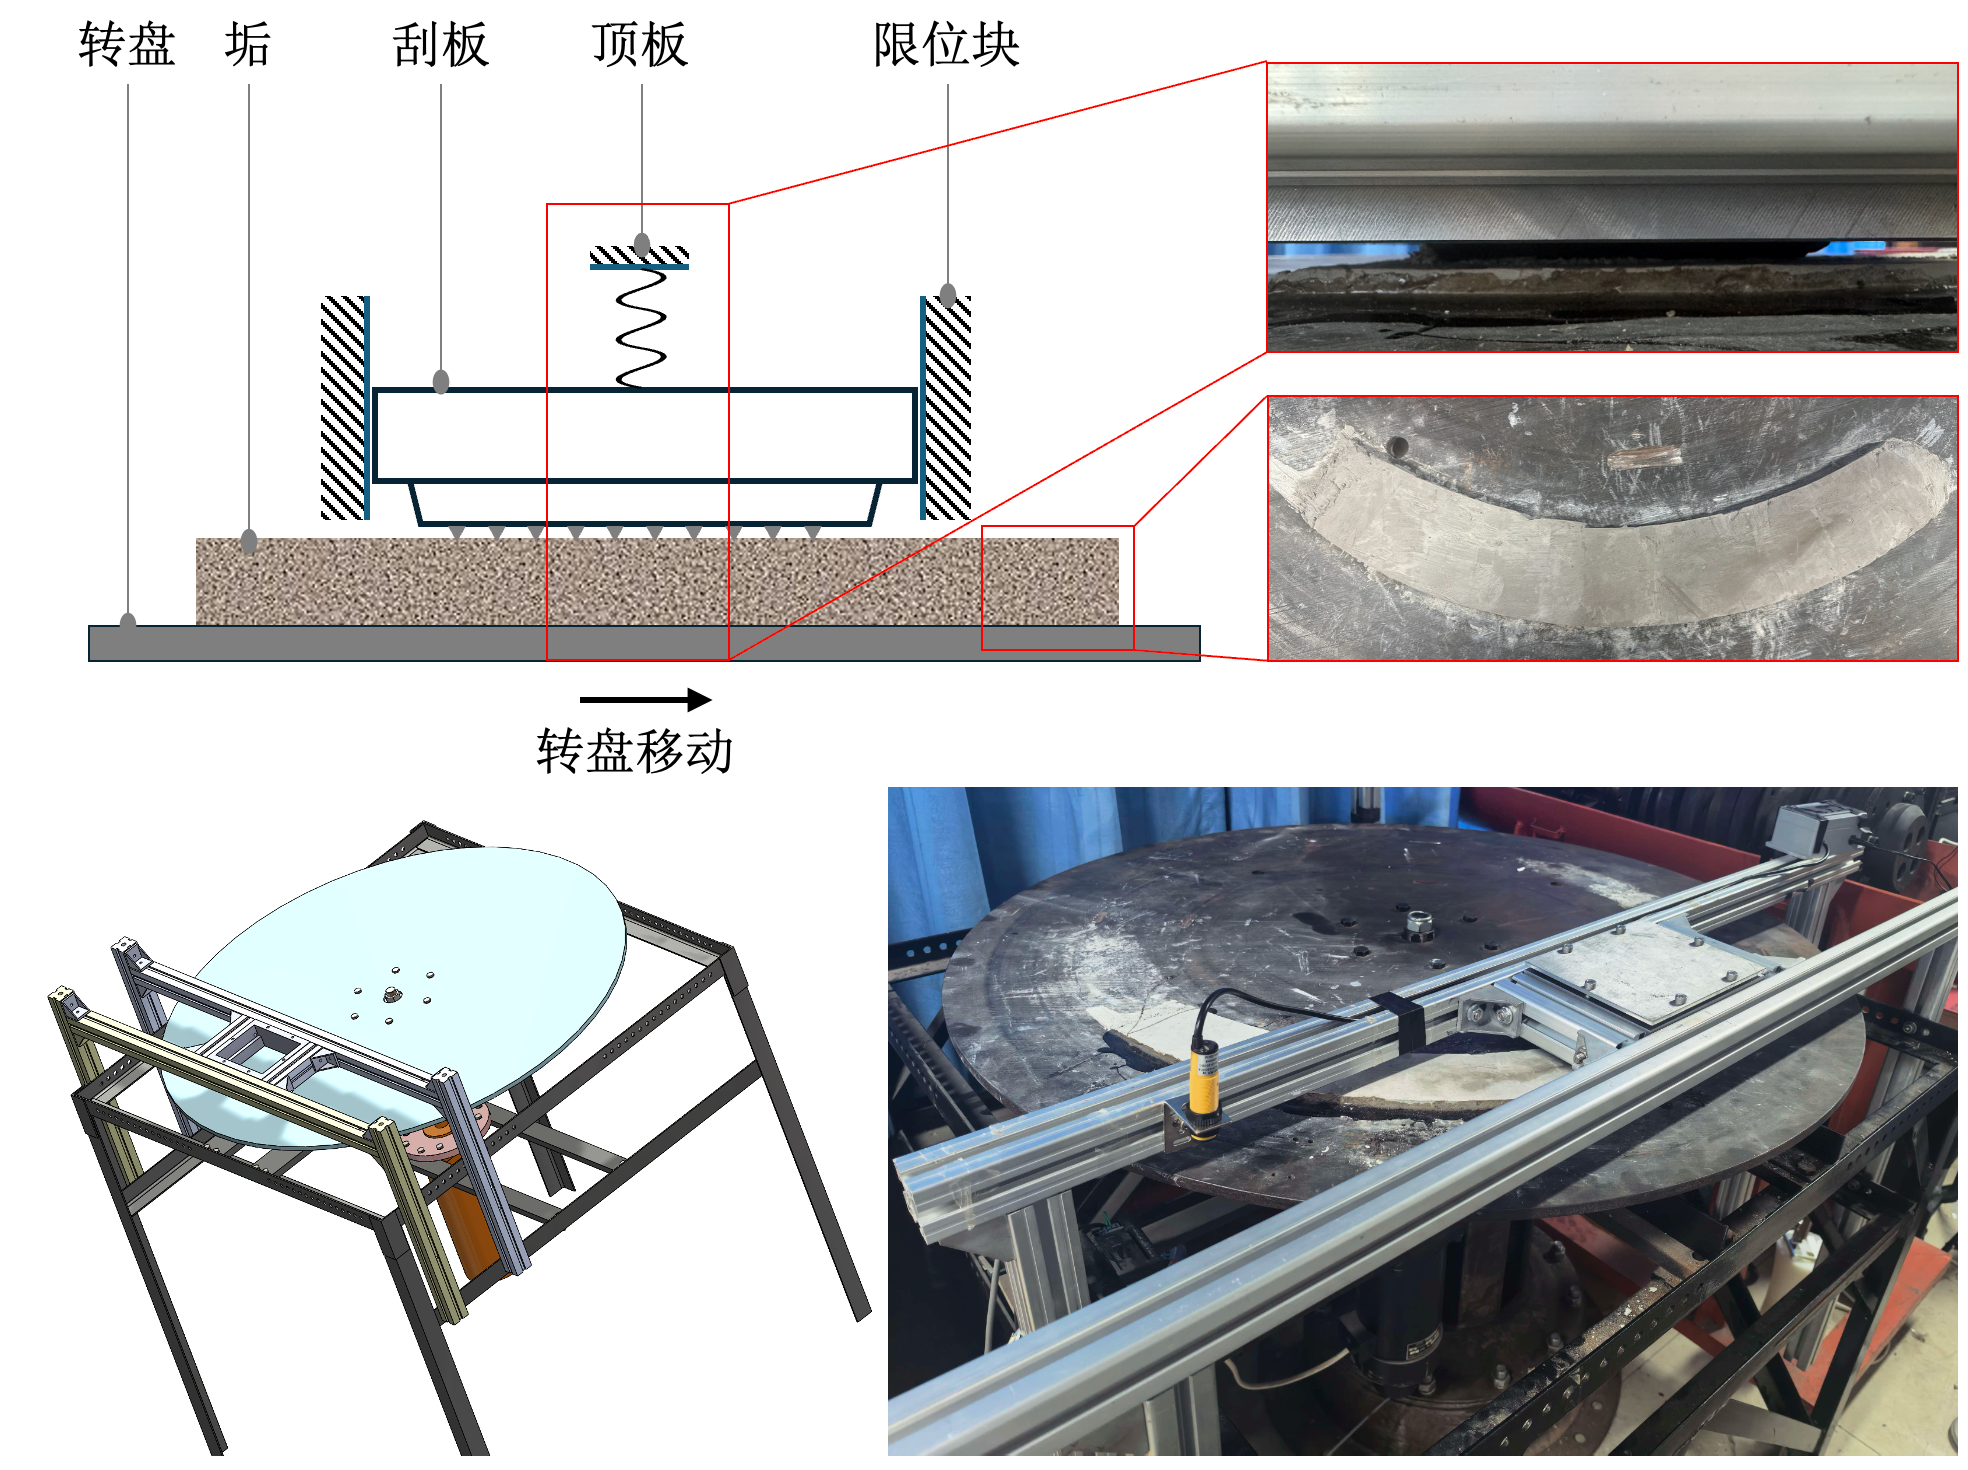
\includegraphics[width=.9\textwidth]{figure/chapter3/scraper-test-rig.png}
	\label{fig:scraper_test_rig_mechanism}
	}
	\vspace{1em}
	\subfloat[弹簧变形量测量原理]{%
	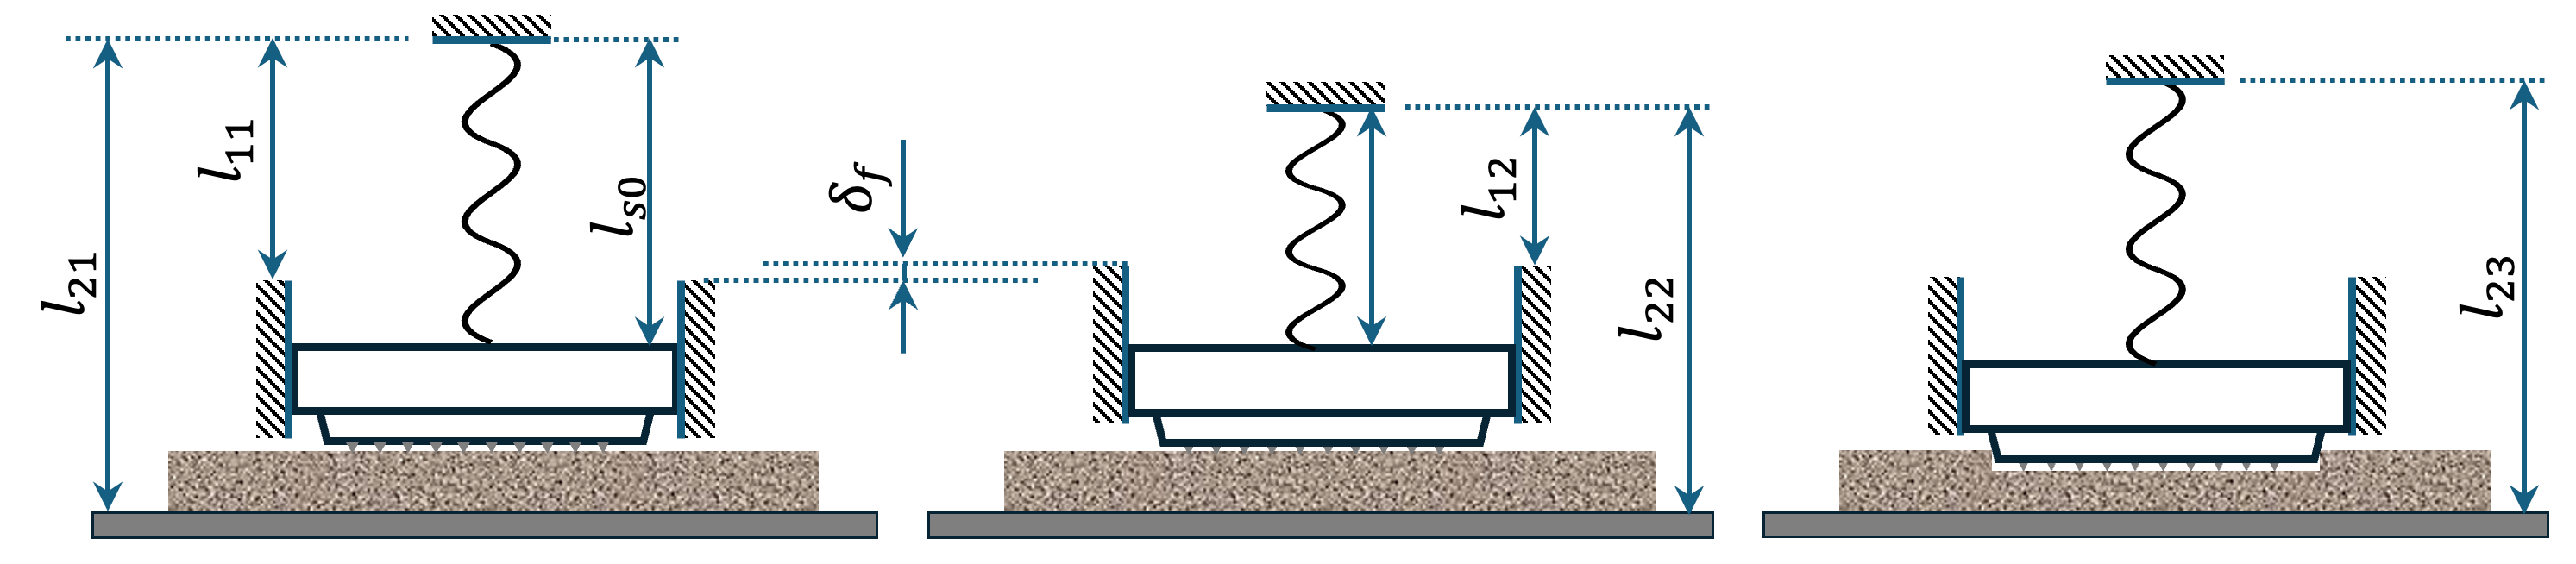
\includegraphics[width=.9\textwidth]{figure/chapter3/scapter-measurement-mechanism.png}
	\label{fig:scapter_measurement_mechanism}
	}
	\caption{刮板刮削性能测试}
	\label{fig:scraper_test_rig}
\end{figure}

试验用垢样为模拟硬垢，其矿物成分以重晶石（硫酸钡）为主，用于近似模拟现场以硫酸钡/钡锶垢为主的坚硬垢层。制作时，将重晶石粉与硫铝酸盐水泥按质量比3:4干混均匀，加水拌合至浆体呈黏糊状态，浇注于放置在转盘盘面上的扇形模具中成形，养护至规定龄期后得到与转盘盘面粘接的扇形垢样。垢样位于距转盘中心半径30\textasciitilde{}38 cm的环形带内（内半径30 cm、外半径38 cm、厚度10 cm），垢样带外缘直径为0.76 m，本装置转盘半径为0.5 m（直径1 m），可满足垢样布置要求；扇形垢样沿周向的包角约为90°。为防止刮削过程中垢样边缘起翘、开裂或整体滑移，每块扇形垢样的两侧边缘均以环氧树脂与转盘盘面粘接固定。环氧树脂固定带及垢样台阶边缘处的刮削状态不具有代表性，故各测量点均布置在扇形垢样中部、距两侧环氧固定带一定距离的区域内，以保证刮削前后测量位置一致。垢样厚度（10 cm）远大于刮削深度（毫米级），刮削过程中垢层可视为半无限厚基体，转盘金属基底对刮削结果的影响可以忽略。为表征垢样的力学属性，同期以相同配比、相同工艺浇注了试块，用于测定垢样的抗压强度与硬度。

刮板是靠弹簧支撑的，为了模拟刮板的这种“浮动”支撑效果，在装置上设置了限位块约束刮板五个运动自由度，保留一个沿盘面法线方向的移动自由度。实验中，限位块用大跨距的横梁与机架固连，在刮板与垢之间的背向力较大时，可能产生挠曲变形$\delta _f$，需在计算弹簧压缩量$\delta_s$时进行补偿。

% 作者待补/核对：①扇形垢样块数及单次刮削流程（包角约90°、转盘半径0.5 m已确认）；②养护条件与龄期；③垢样抗压强度、硬度实测值及正文引用处；④刮刀刀齿沿运动方向接触宽度w的量级（正文按“毫米至厘米、垂向偏差不超过0.1 mm”定性表述，若实测请补具体值）；⑤手拉线速度0.05 m/s的测量位置（正文按接触区平均半径33.5 cm处表述）；⑥各尺寸测量基准面是否统一取垢样顶面。
实验记录的数据含义如图\ref{fig:scapter_measurement_mechanism}所示。实验前，先让弹簧处于原长状态，测量距离$l_{11}$和$l_{21}$，这两个尺寸分别是顶板顶部测量基面和限位块顶部、转盘盘面之间的距离。然后，根据弹簧的参考压缩量，将弹簧预紧，测量$l_{11}$、$l_{21}$，记为$l_{12}$、$l_{22}$。转动转盘，使刮板完成一次刮削过程，停止设备后，再次测量尺寸$l_{21}$，记为$l_{23}$。从实验台上取一个参考位置，在划痕的两侧取两个监测点，测量监测点相对于参考位置之间的距离$l_{31}$、$l_{32}$，再测量刮削坑的底部与参考点之间的距离$l_4$。实验中的尺寸测量采用的是精度为0.02 mm的游标卡尺，且刮削前后的尺寸测量均在同一扇形垢样区、同一测量位置完成，以保证测量基准一致。



根据几何关系，单次刮削产生的坑深度$\delta_c$、坑的累积深度$\delta_c'$，弹簧压缩量估计值$\delta_s$为
\begin{equation}
\centering
	\begin{aligned}
		\delta_c' & =l_4-\frac{l_{31}+l_{32}}{2}\\
		\delta_f & = l_{23}-l_{21}  \\ 
		\delta_s & = l_{11}-l_{12} - \delta_f- \delta_c'
	\end{aligned}
\end{equation}

垢经刮削后的形貌如图\ref{fig:scale_profile}所示。刮板前刀面附近堆积有粉末状和崩碎状屑，刀齿的容屑槽中也有此类屑，由此证明，所设计的刮板能有效刮除硬垢。在刮削区域的边缘也有这样的屑。从切屑的性质可以推测出，所设计的垢为脆性垢，与文献所述的垢性质吻合。%补充是哪一篇文献
从图中还可以看出，产屑量与弹簧的压缩量成正相关。
\begin{figure}[htbp]
	\centering
	\subfloat[$\delta_s=3.095\textrm{mm}$]{%
	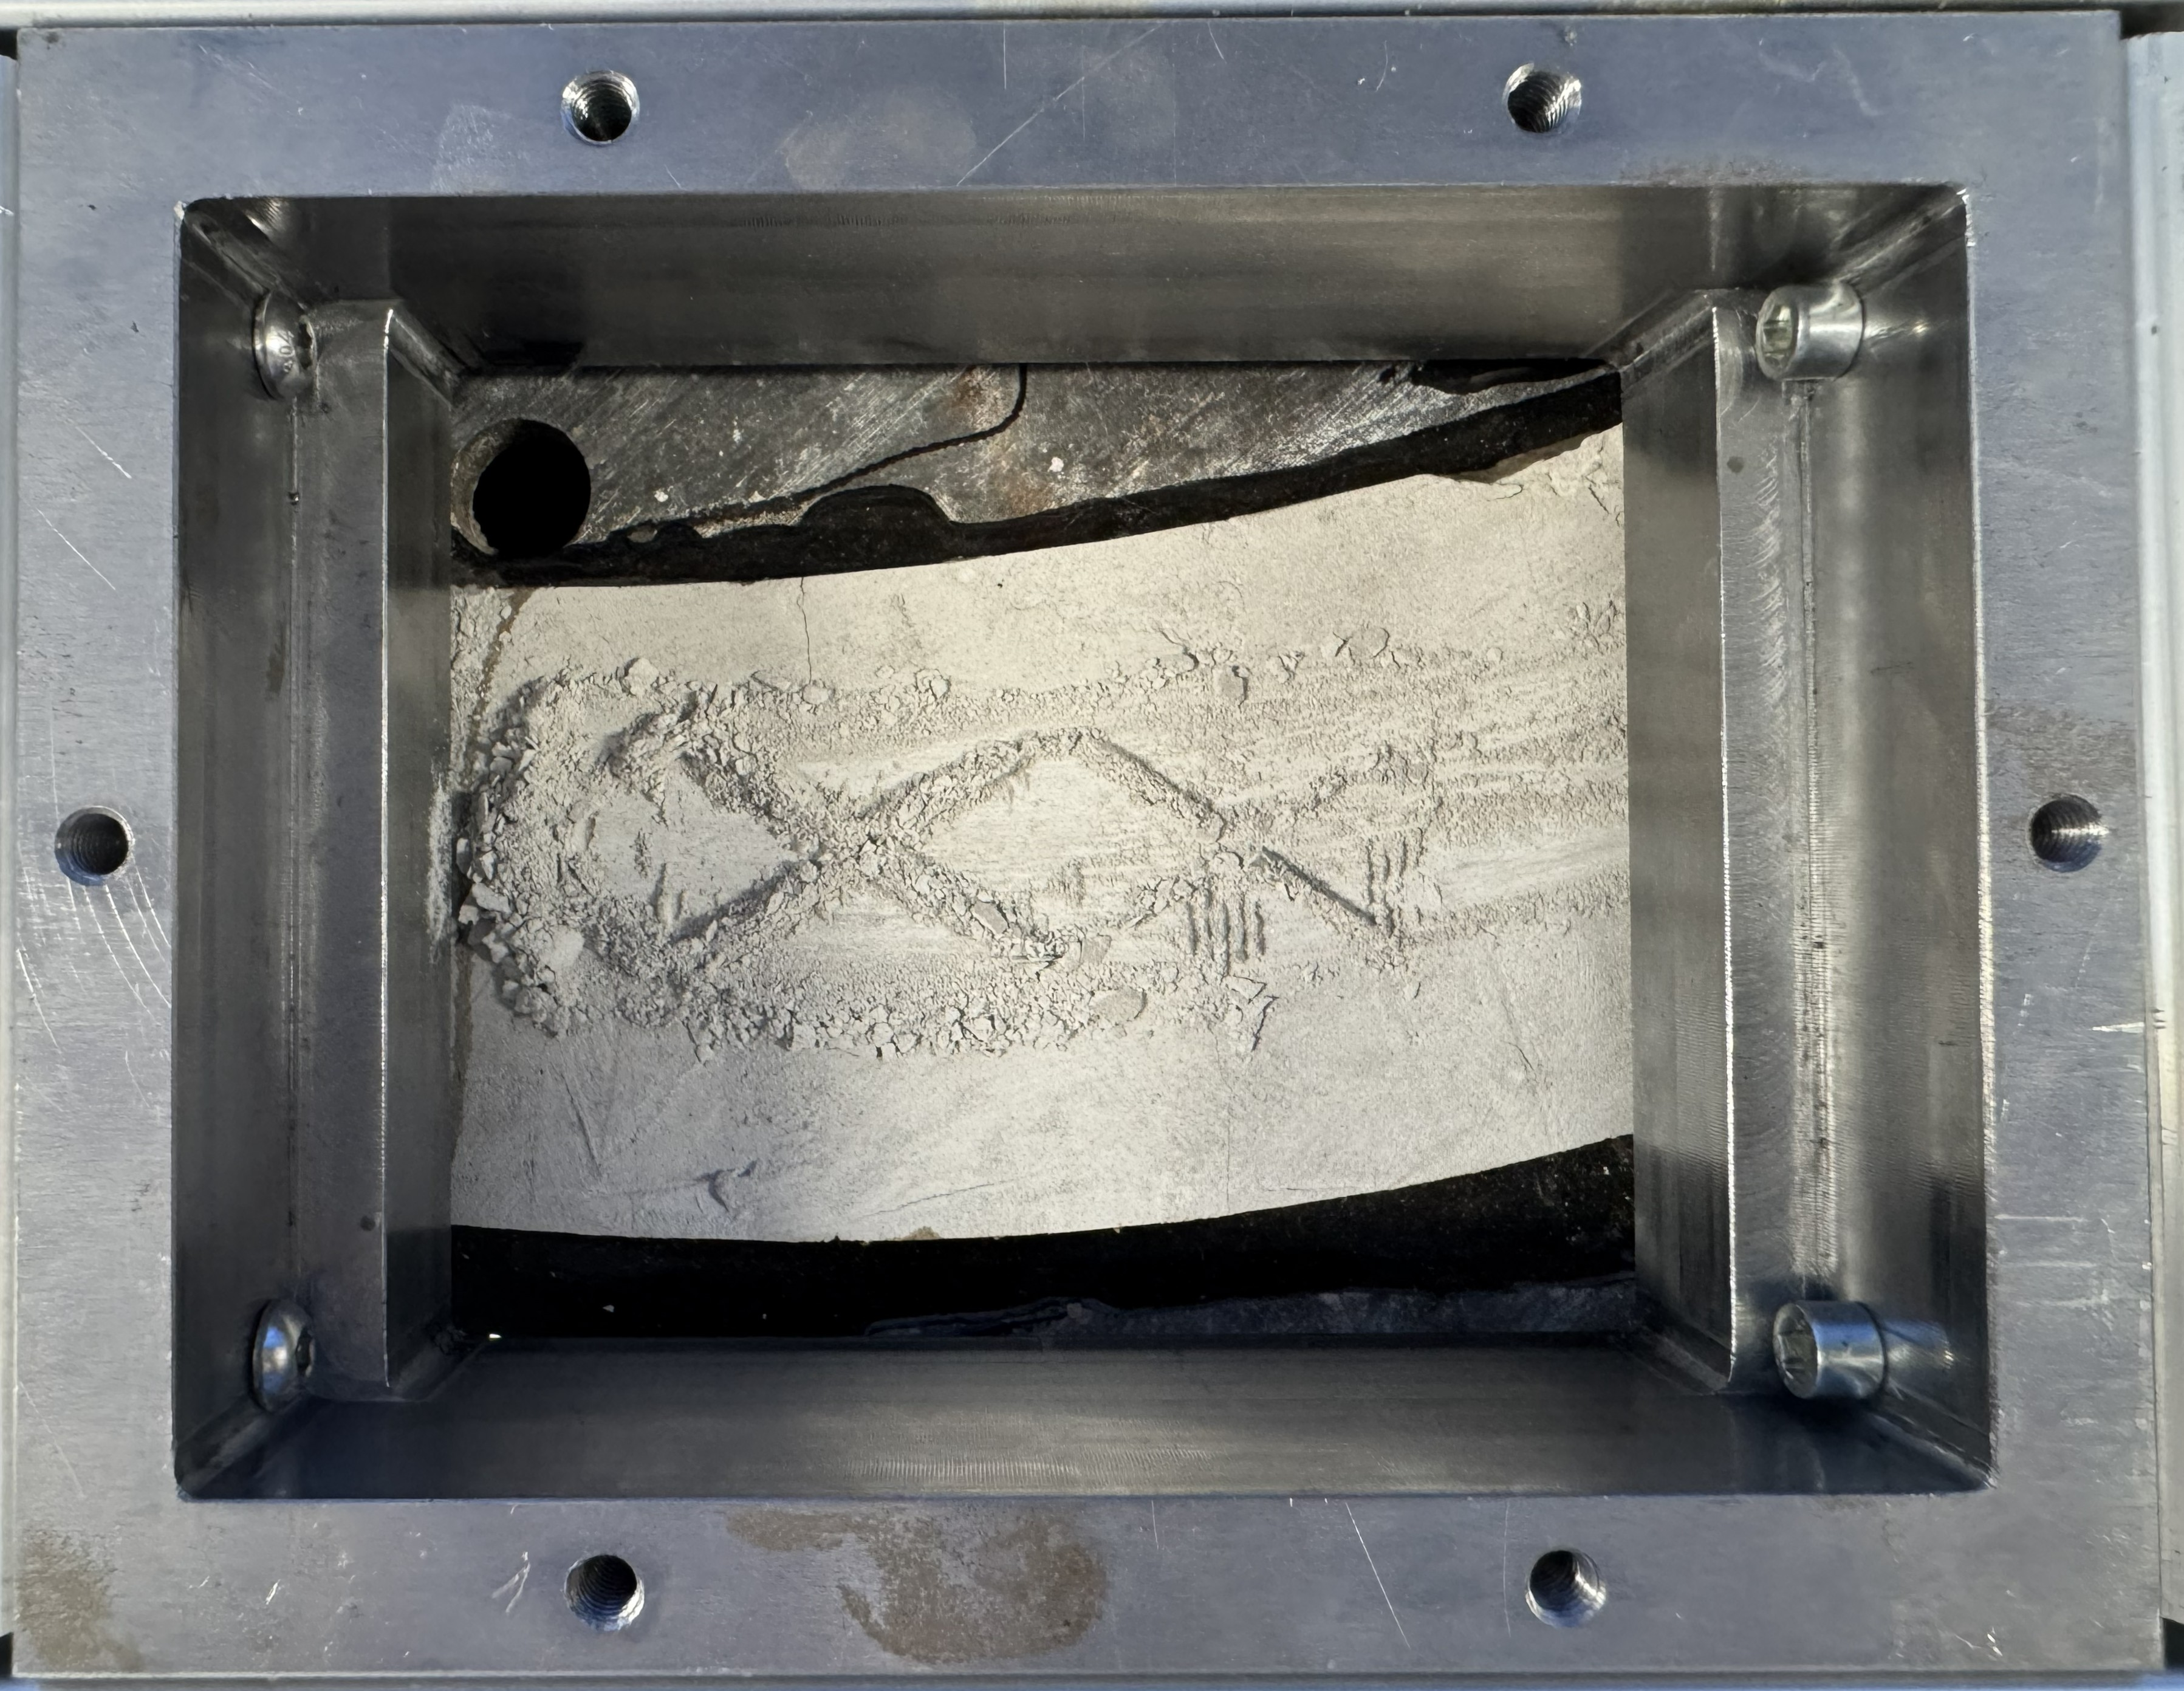
\includegraphics[height=4.0cm]{figure/chapter3/scale-1.jpg}
	\label{fig:scale_1}
	}
	%\hfill
	\subfloat[$\delta_s=4.875\textrm{mm}$]{%
	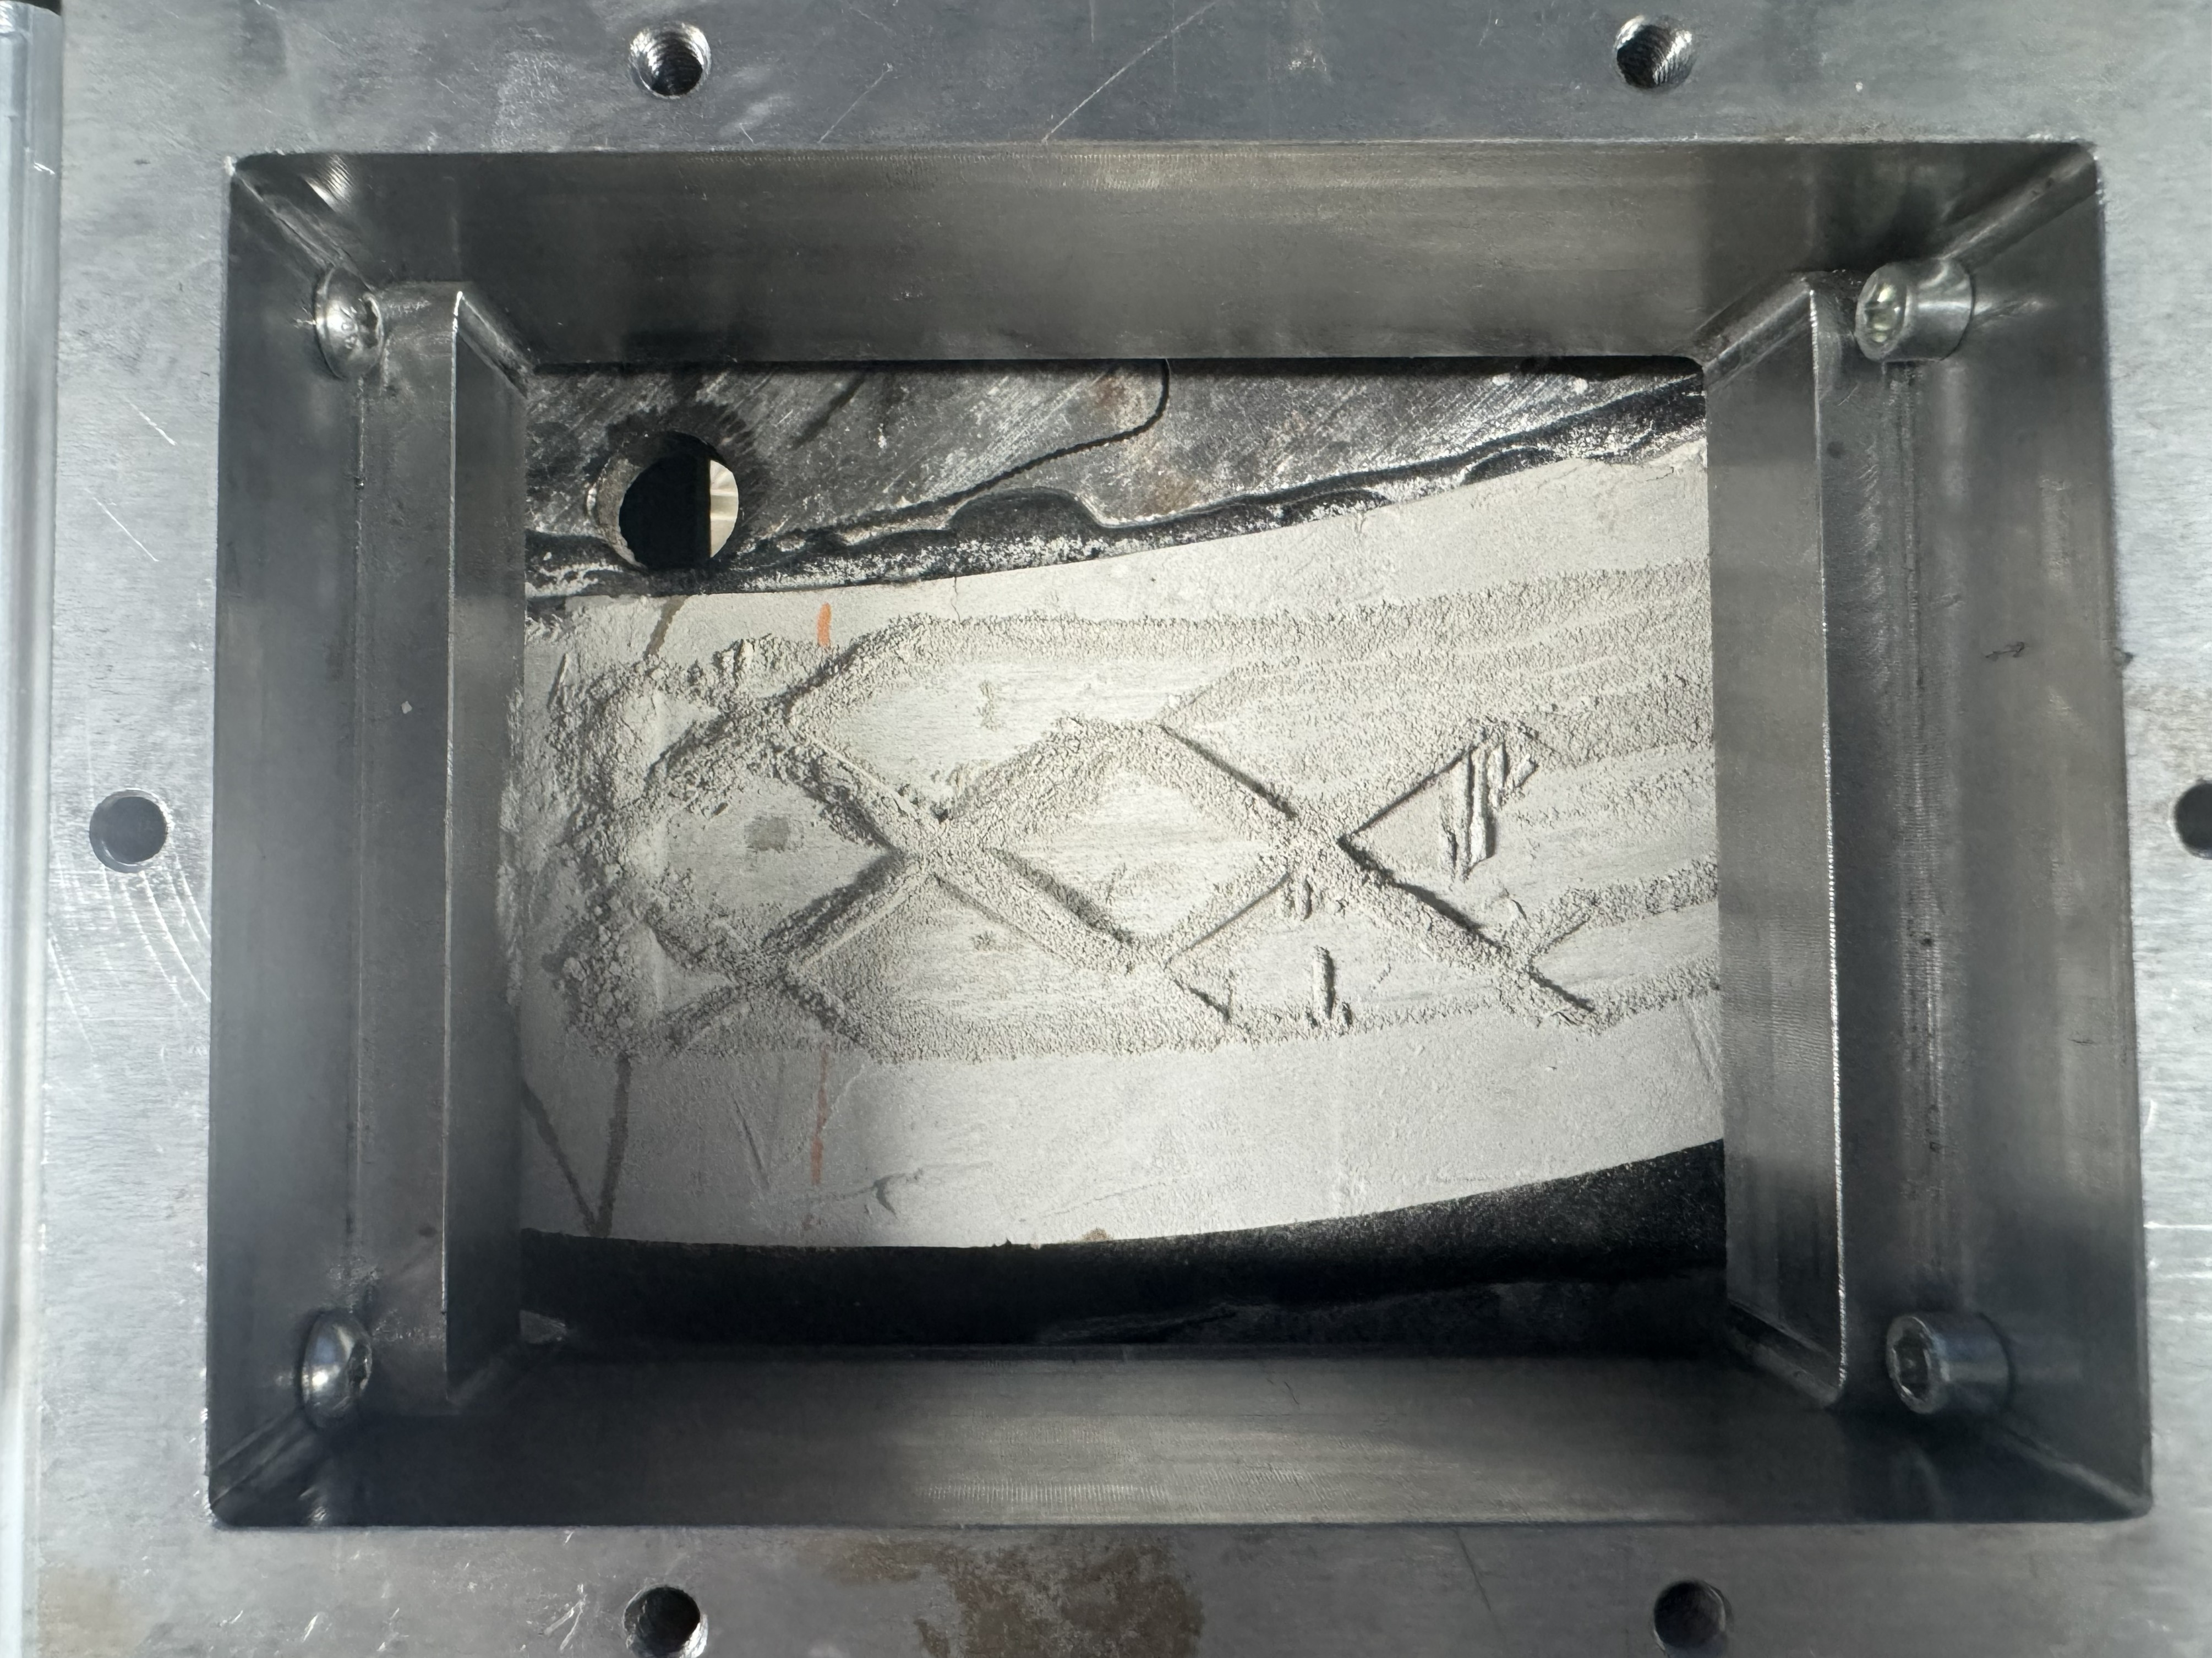
\includegraphics[height=4.0cm]{figure/chapter3/scale-4.jpg}
	\label{fig:scale_4}
	}
	\\[1.2em]
	\subfloat[$\delta_s=5.155\textrm{mm}$]{%
	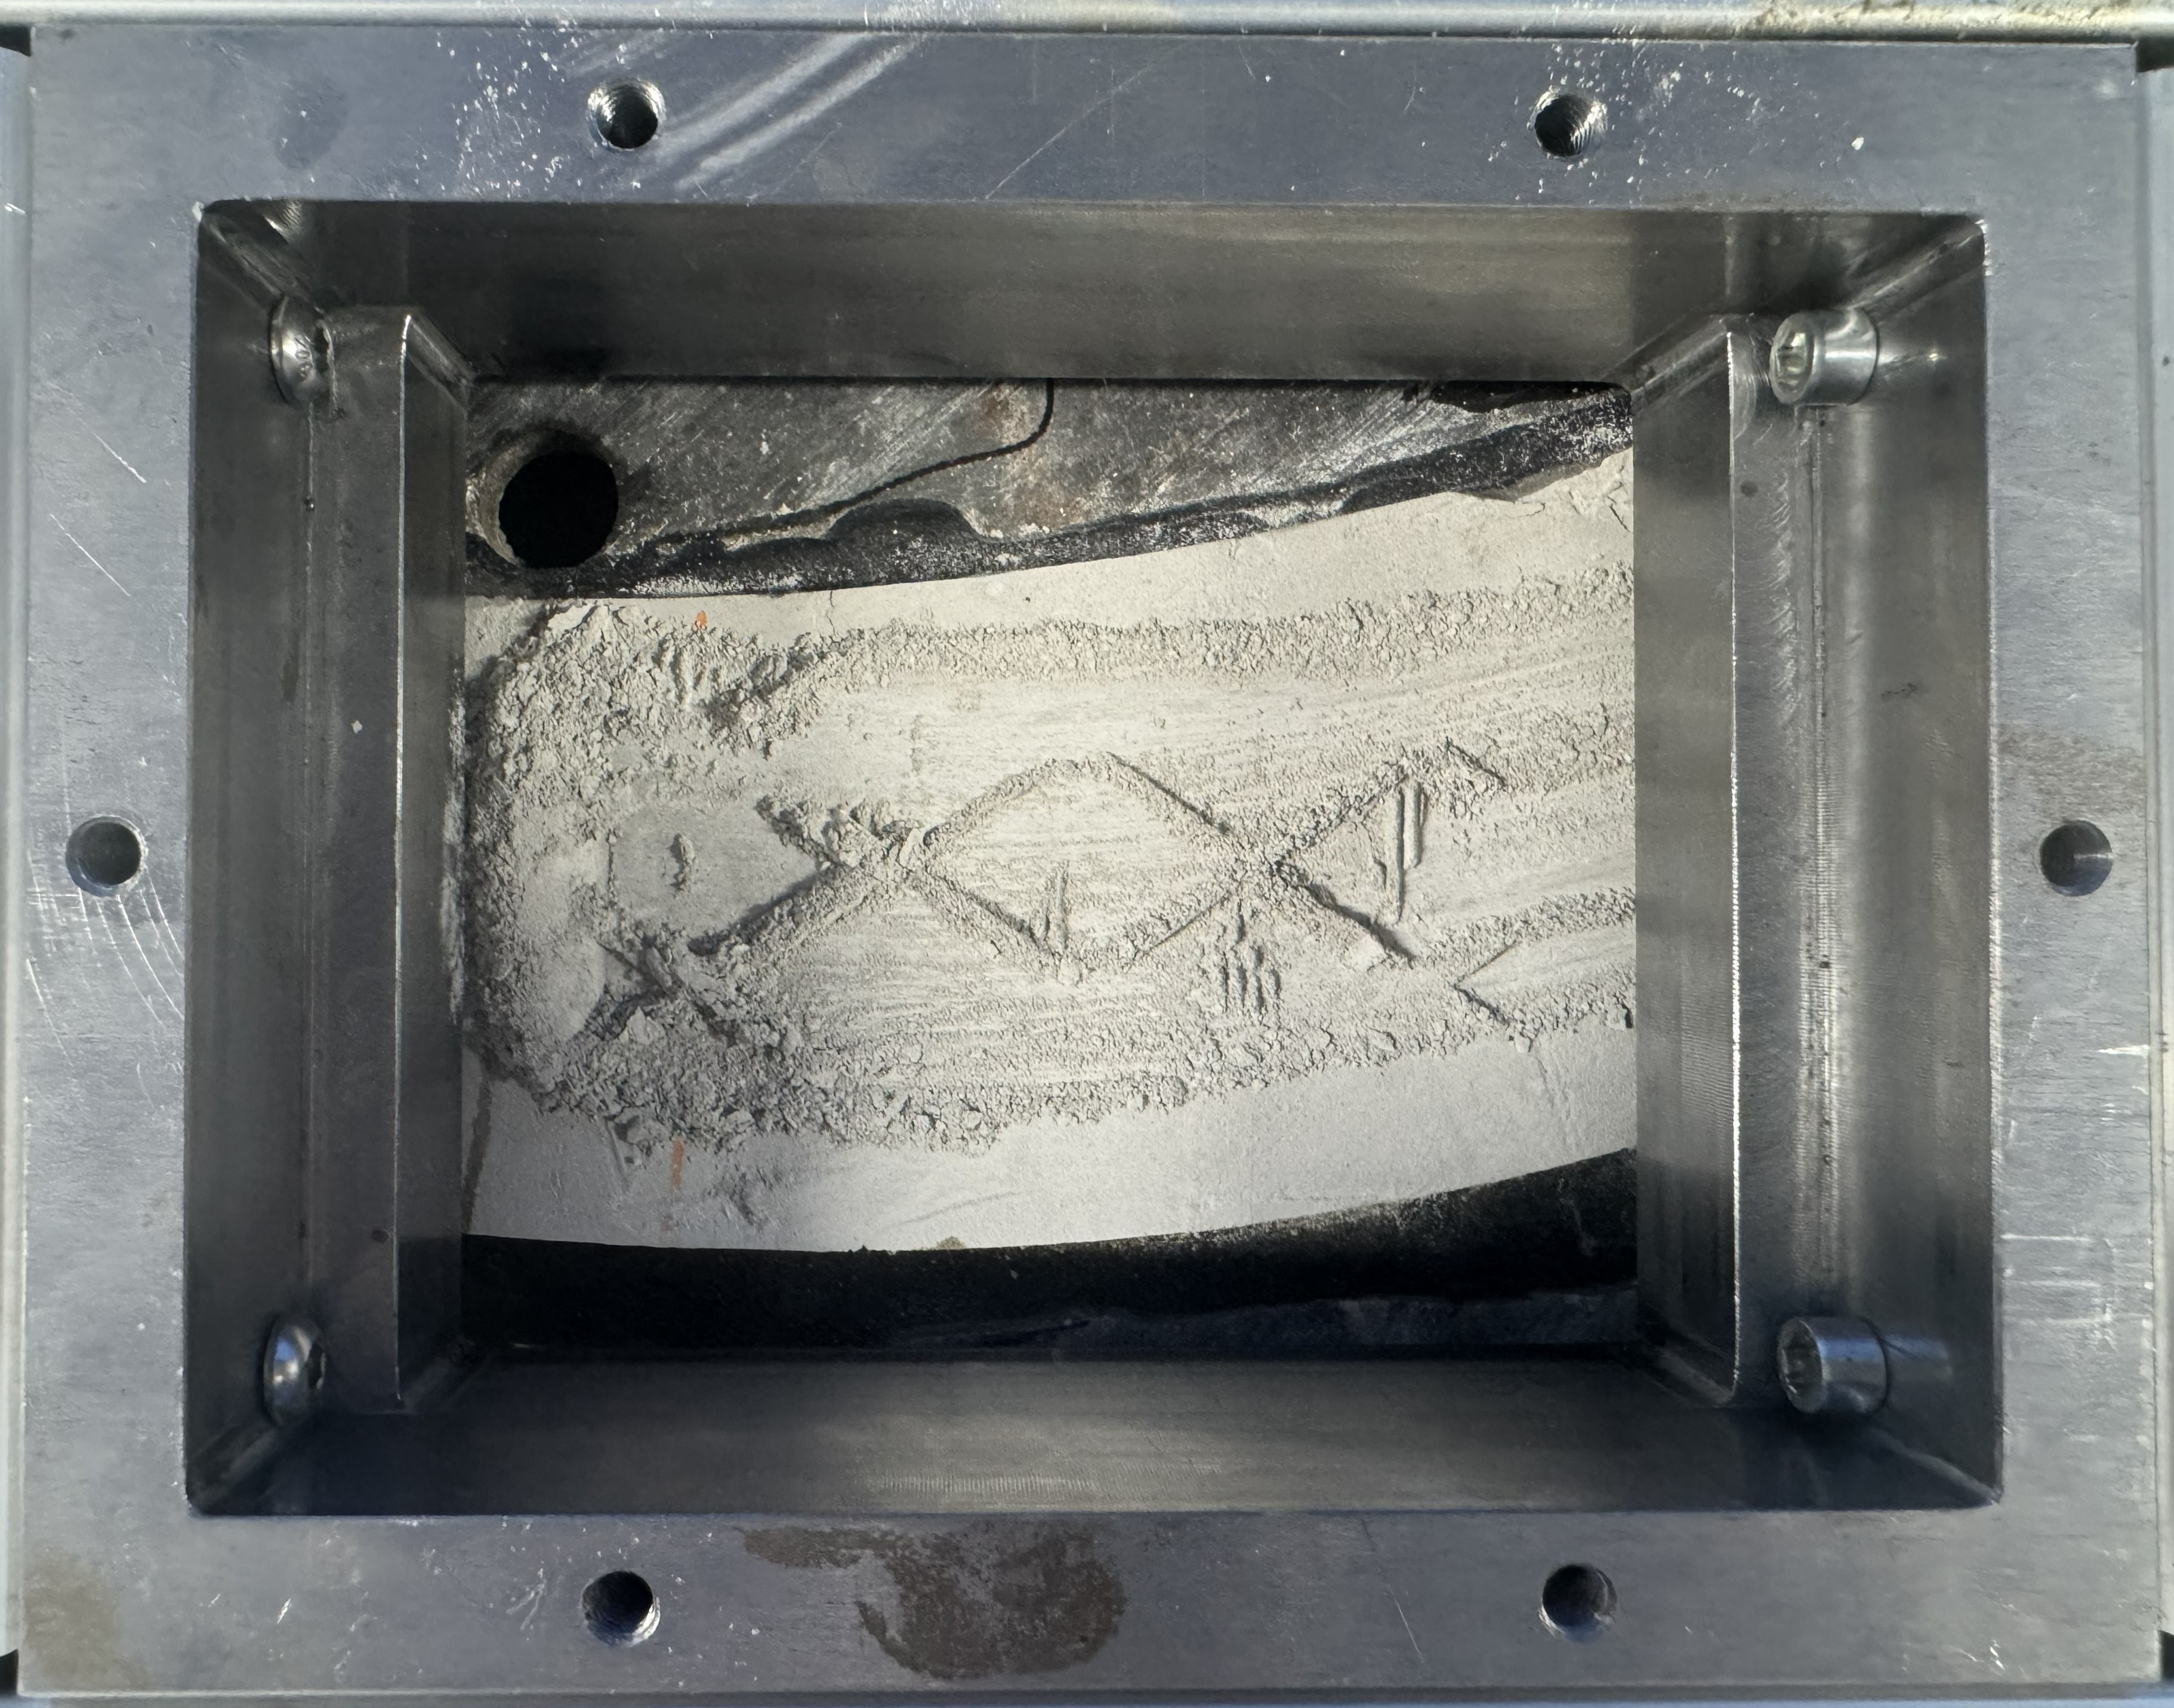
\includegraphics[height=4.0cm]{figure/chapter3/scale-3.jpg}
	\label{fig:scale_3}
	}
	%\hfill
	\subfloat[$\delta_s=6.465\textrm{mm}$]{%
	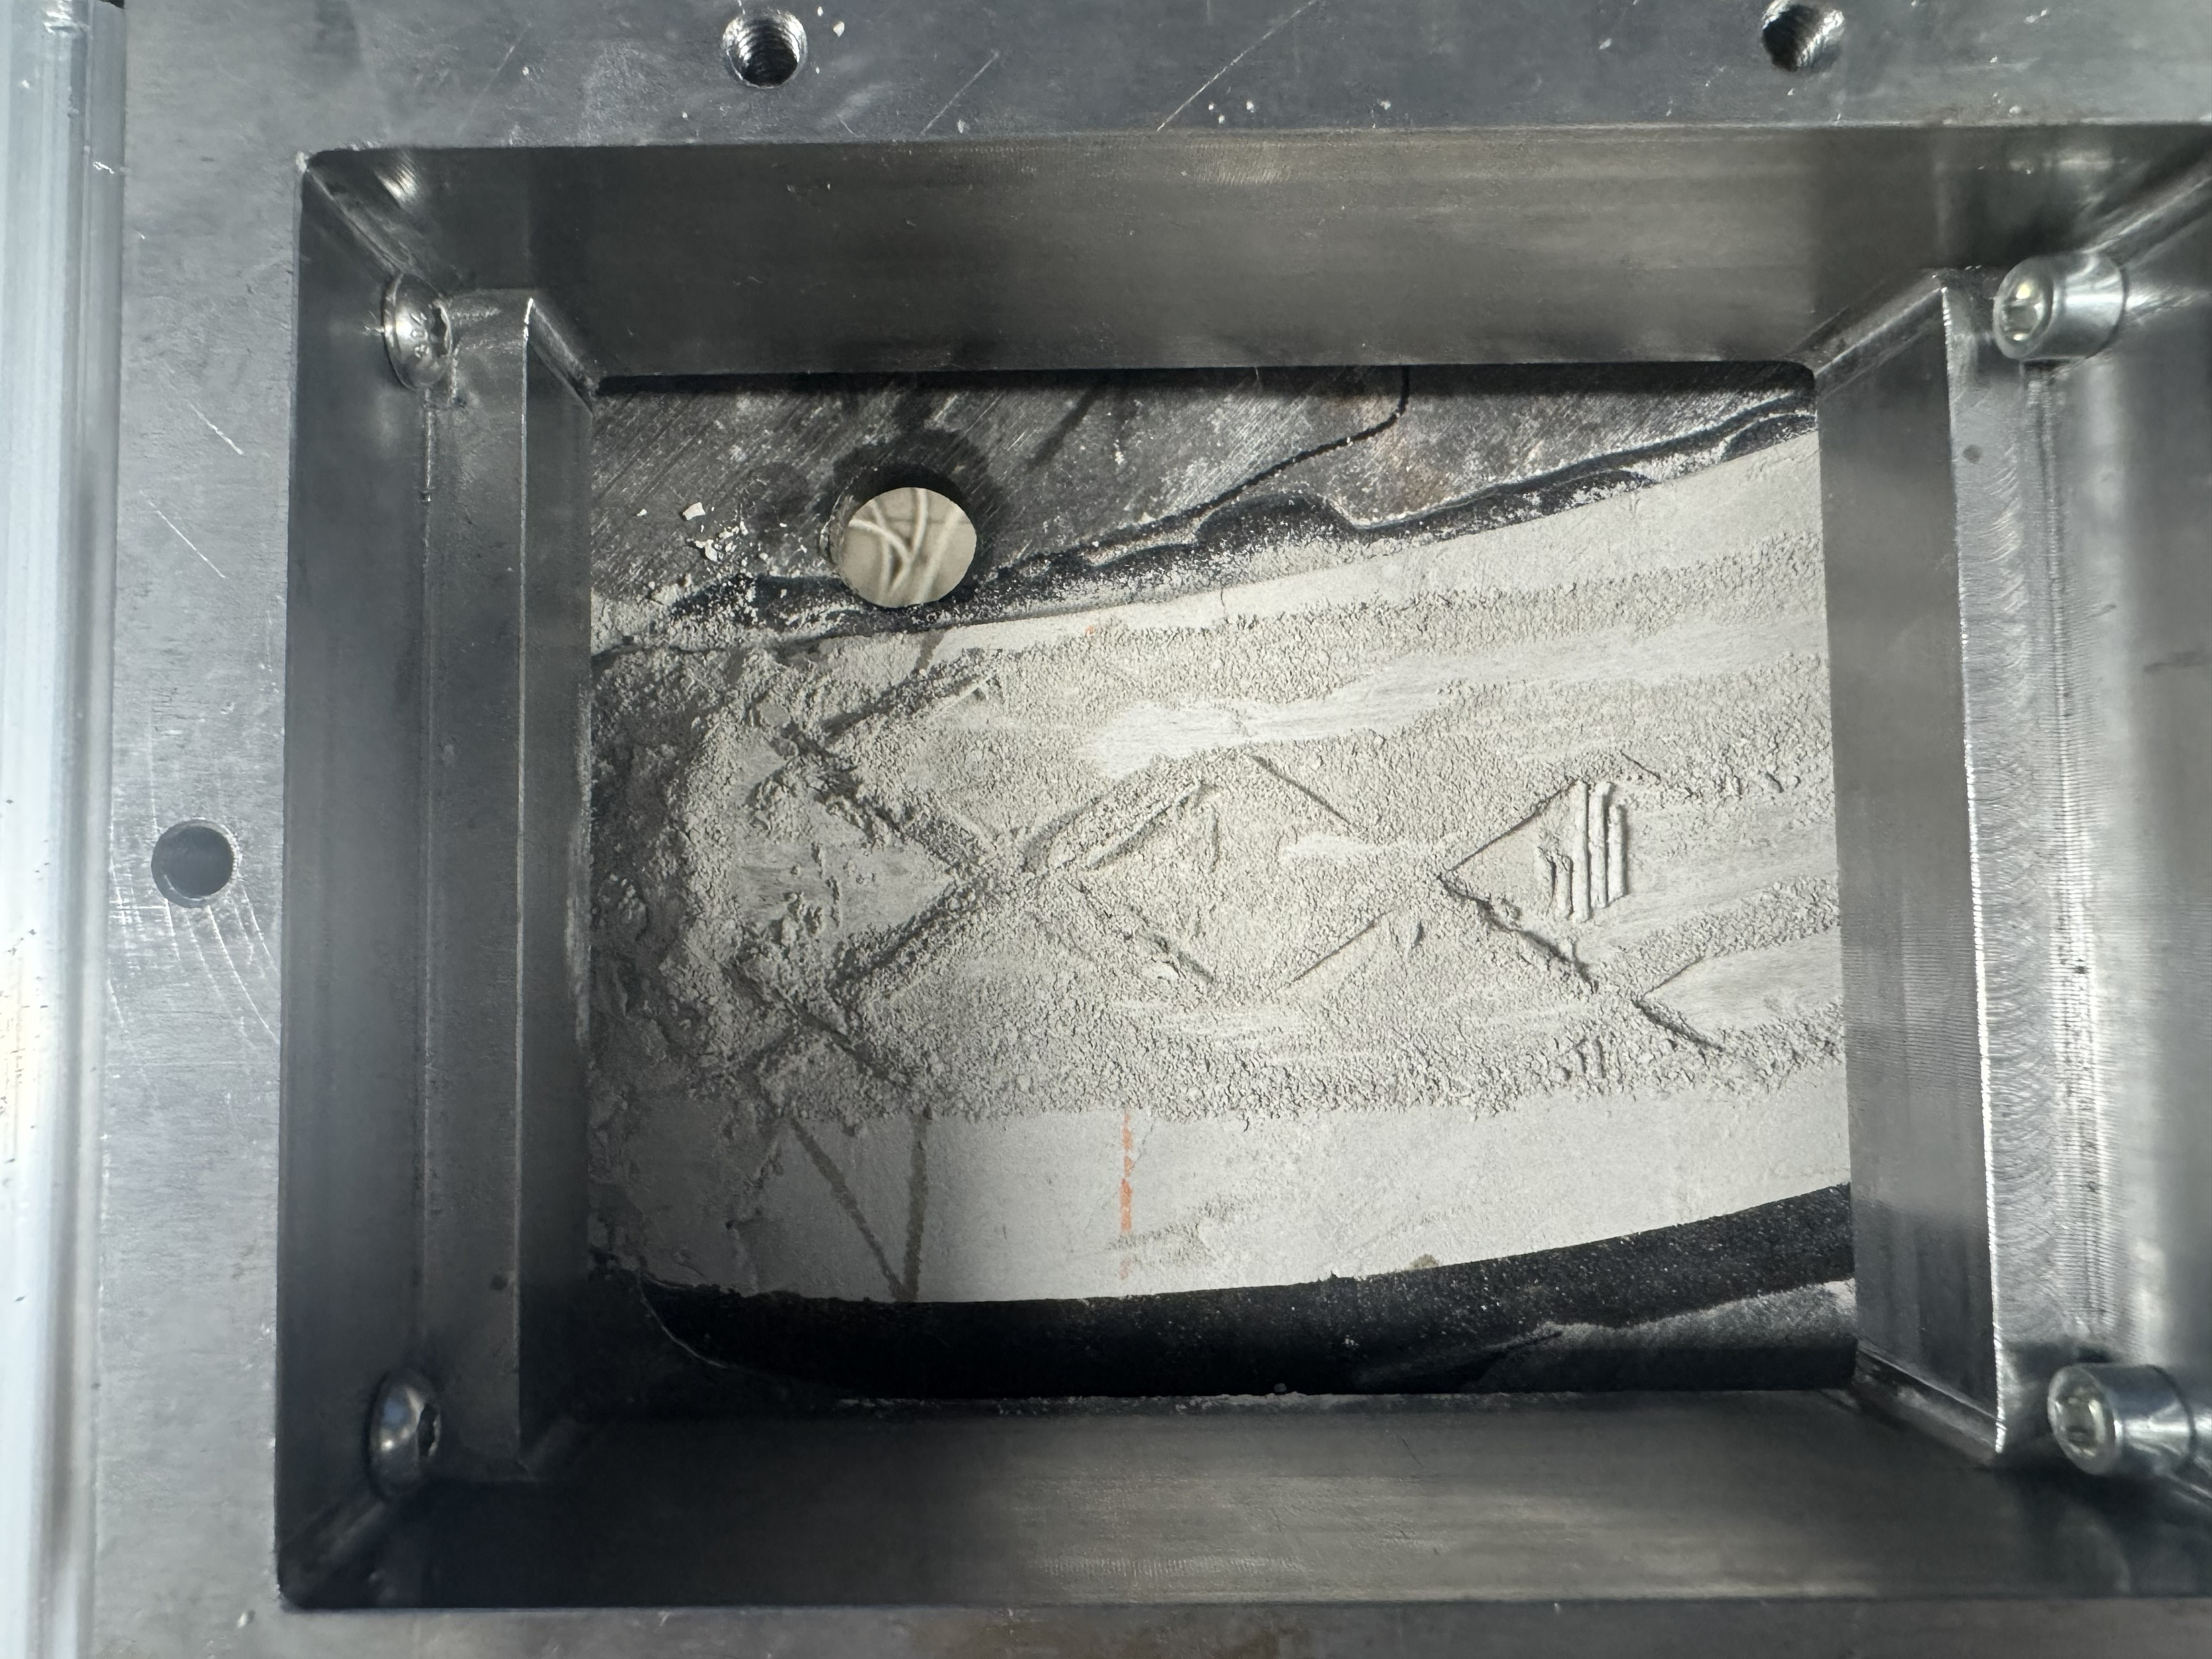
\includegraphics[height=4.0cm]{figure/chapter3/scale-5.jpg}
	\label{fig:scale_5}
	}	
	\caption{垢层经刮削后的表面形貌（不同弹簧压缩量）}
	\label{fig:scale_profile}
\end{figure}


此外，刮板表面的有效刮削功能单元是表面齿，总体上看，刮板主要依靠具有负前角的前刀面进行刮削，其余位置的齿起到辅助作用。刮削中产生的粉末状垢屑极易导致刮板上刀齿前刀面堵塞，如图\ref{fig:scraper_profile}所示。在清理垢时还发现，后刀面在弹簧的巨大预紧力作用下与垢强烈摩擦，后刀面附着有一层质地坚硬的垢变质层，其强度和硬度比垢基材高，在一定程度上减缓了后刀面的磨损。刮板前刀面附近的切削齿堵塞较为严重，增加弹簧的预紧力会加剧这种堵塞效果，这说明此刮板应容易堵塞。横向螺纹齿最容易被堵塞，斜向的三角齿由于容屑槽空间大，切削性能可保持的时间会更长。在实际应用中，可以推测，螺纹齿在刮削的初期就被堵塞而失效。主切削齿在初始阶段承担主要的刮削任务；随着刮削行程的增长，其主切削刃磨钝，三角齿主要起着刮削的作用。在实际应用中，如能建立循环不断冲洗刮板，将有助于屑从容屑槽中排出，对提高刮板的使用效能有促进作用。

\begin{figure}[htbp]
	\centering
	\subfloat[$\delta_s=3.095\textrm{mm}$]{%
	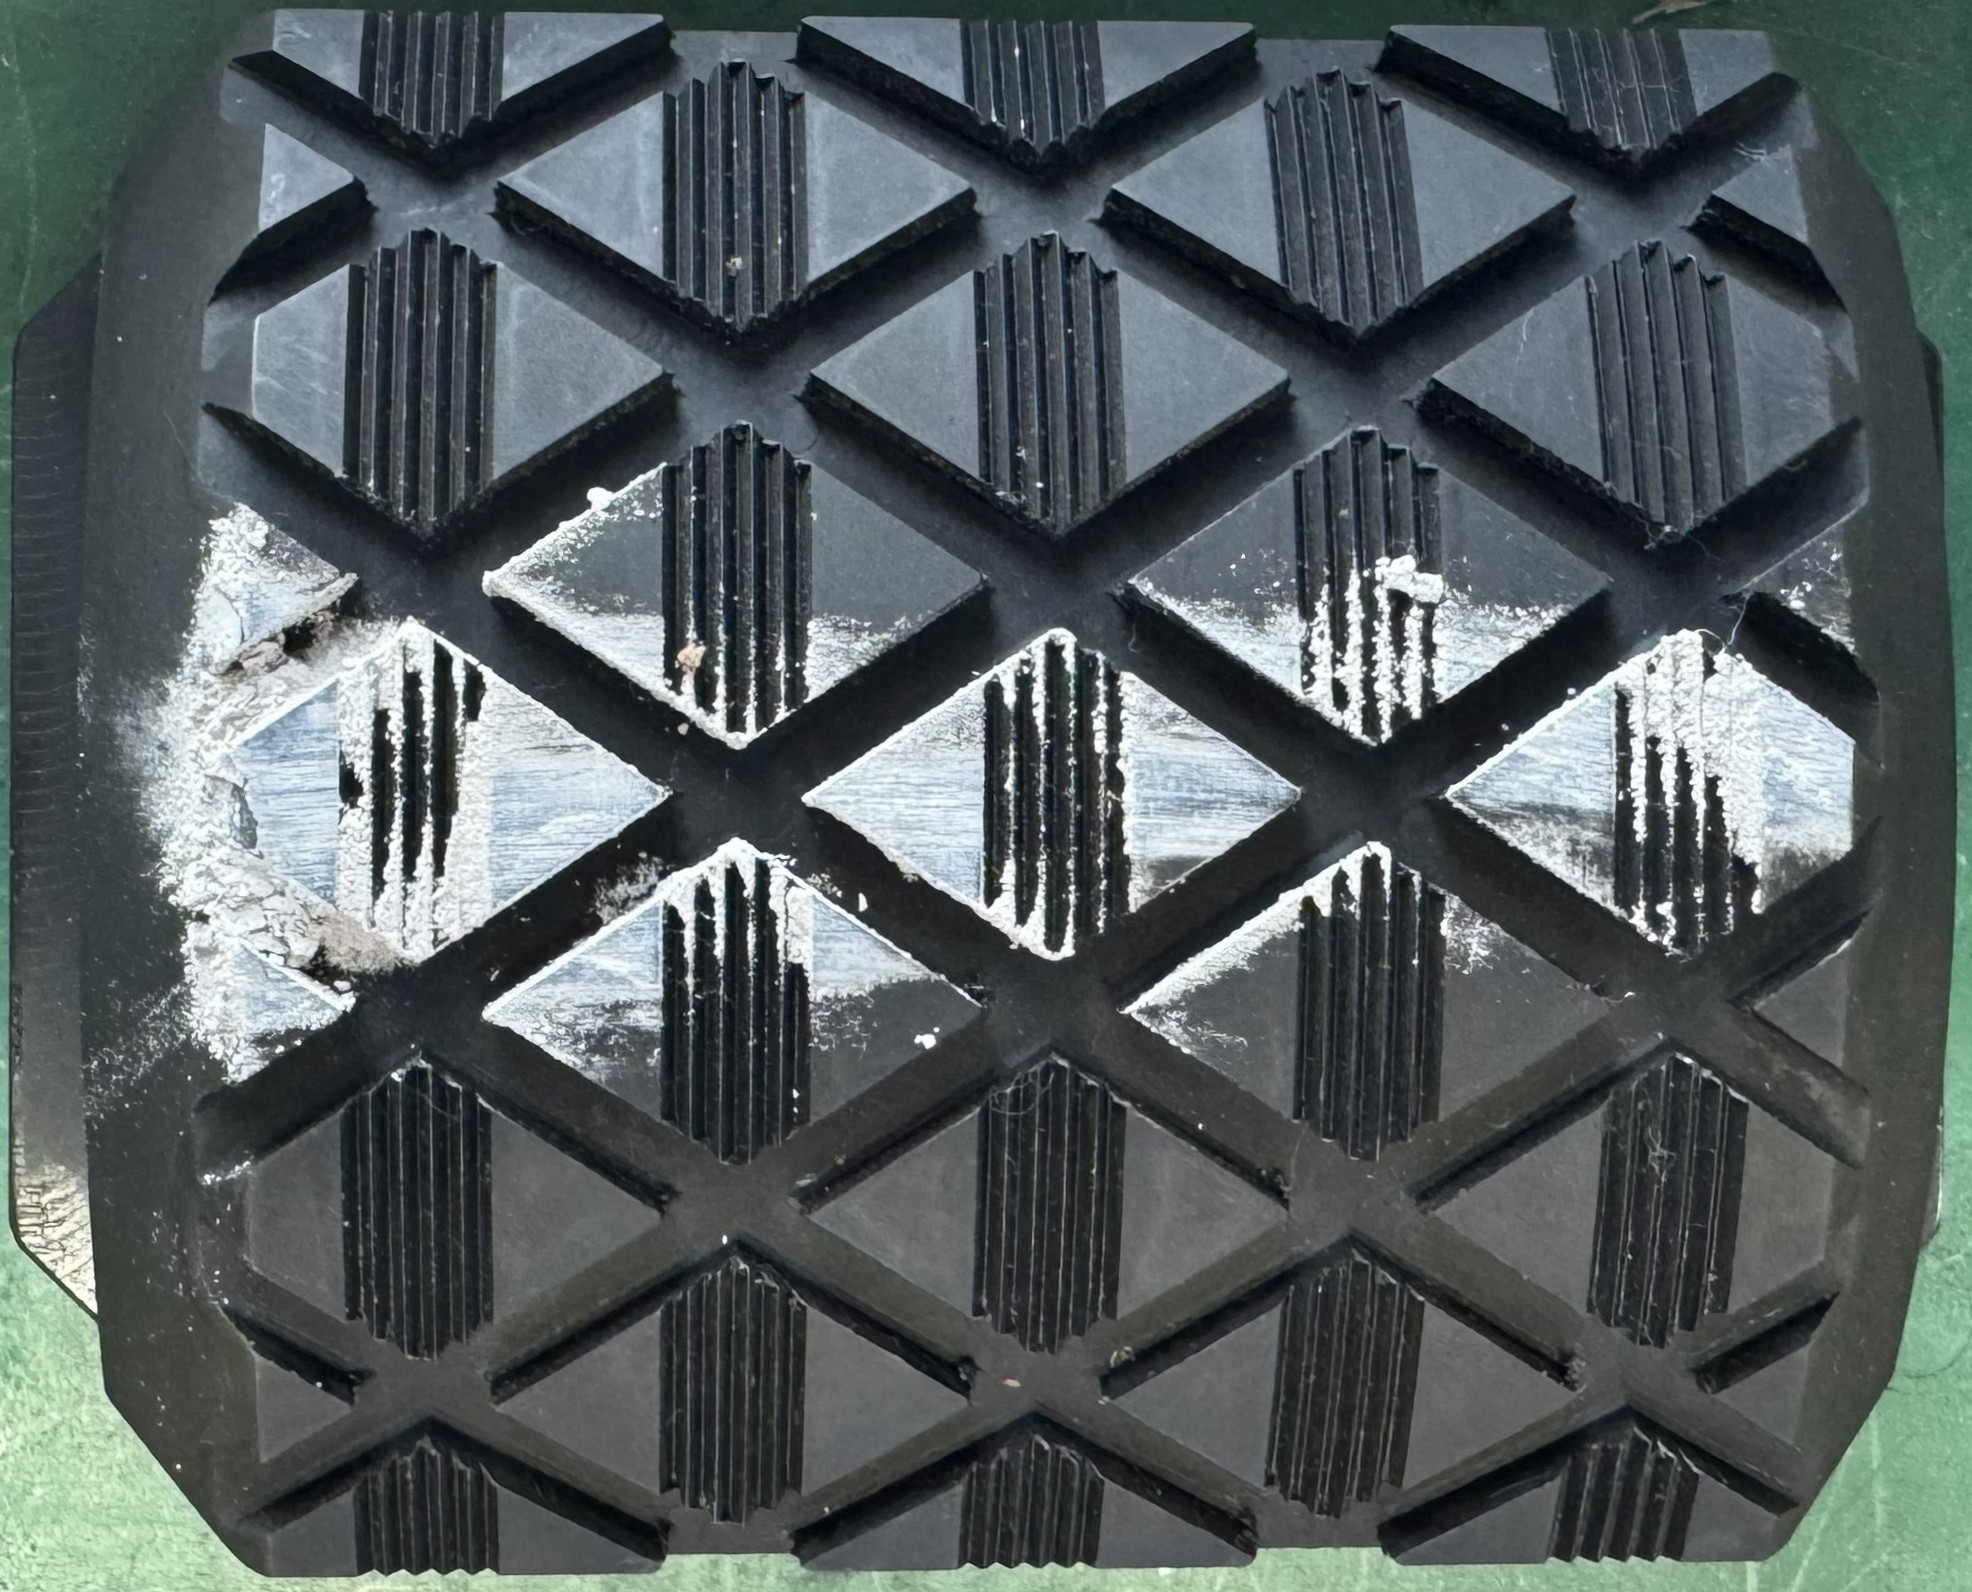
\includegraphics[width=.32\textwidth]{figure/chapter3/scraper-1.jpg}
	\label{fig:scraper_1}
	}
	%\hfill
	\subfloat[$\delta_s=4.875\textrm{mm}$]{%
	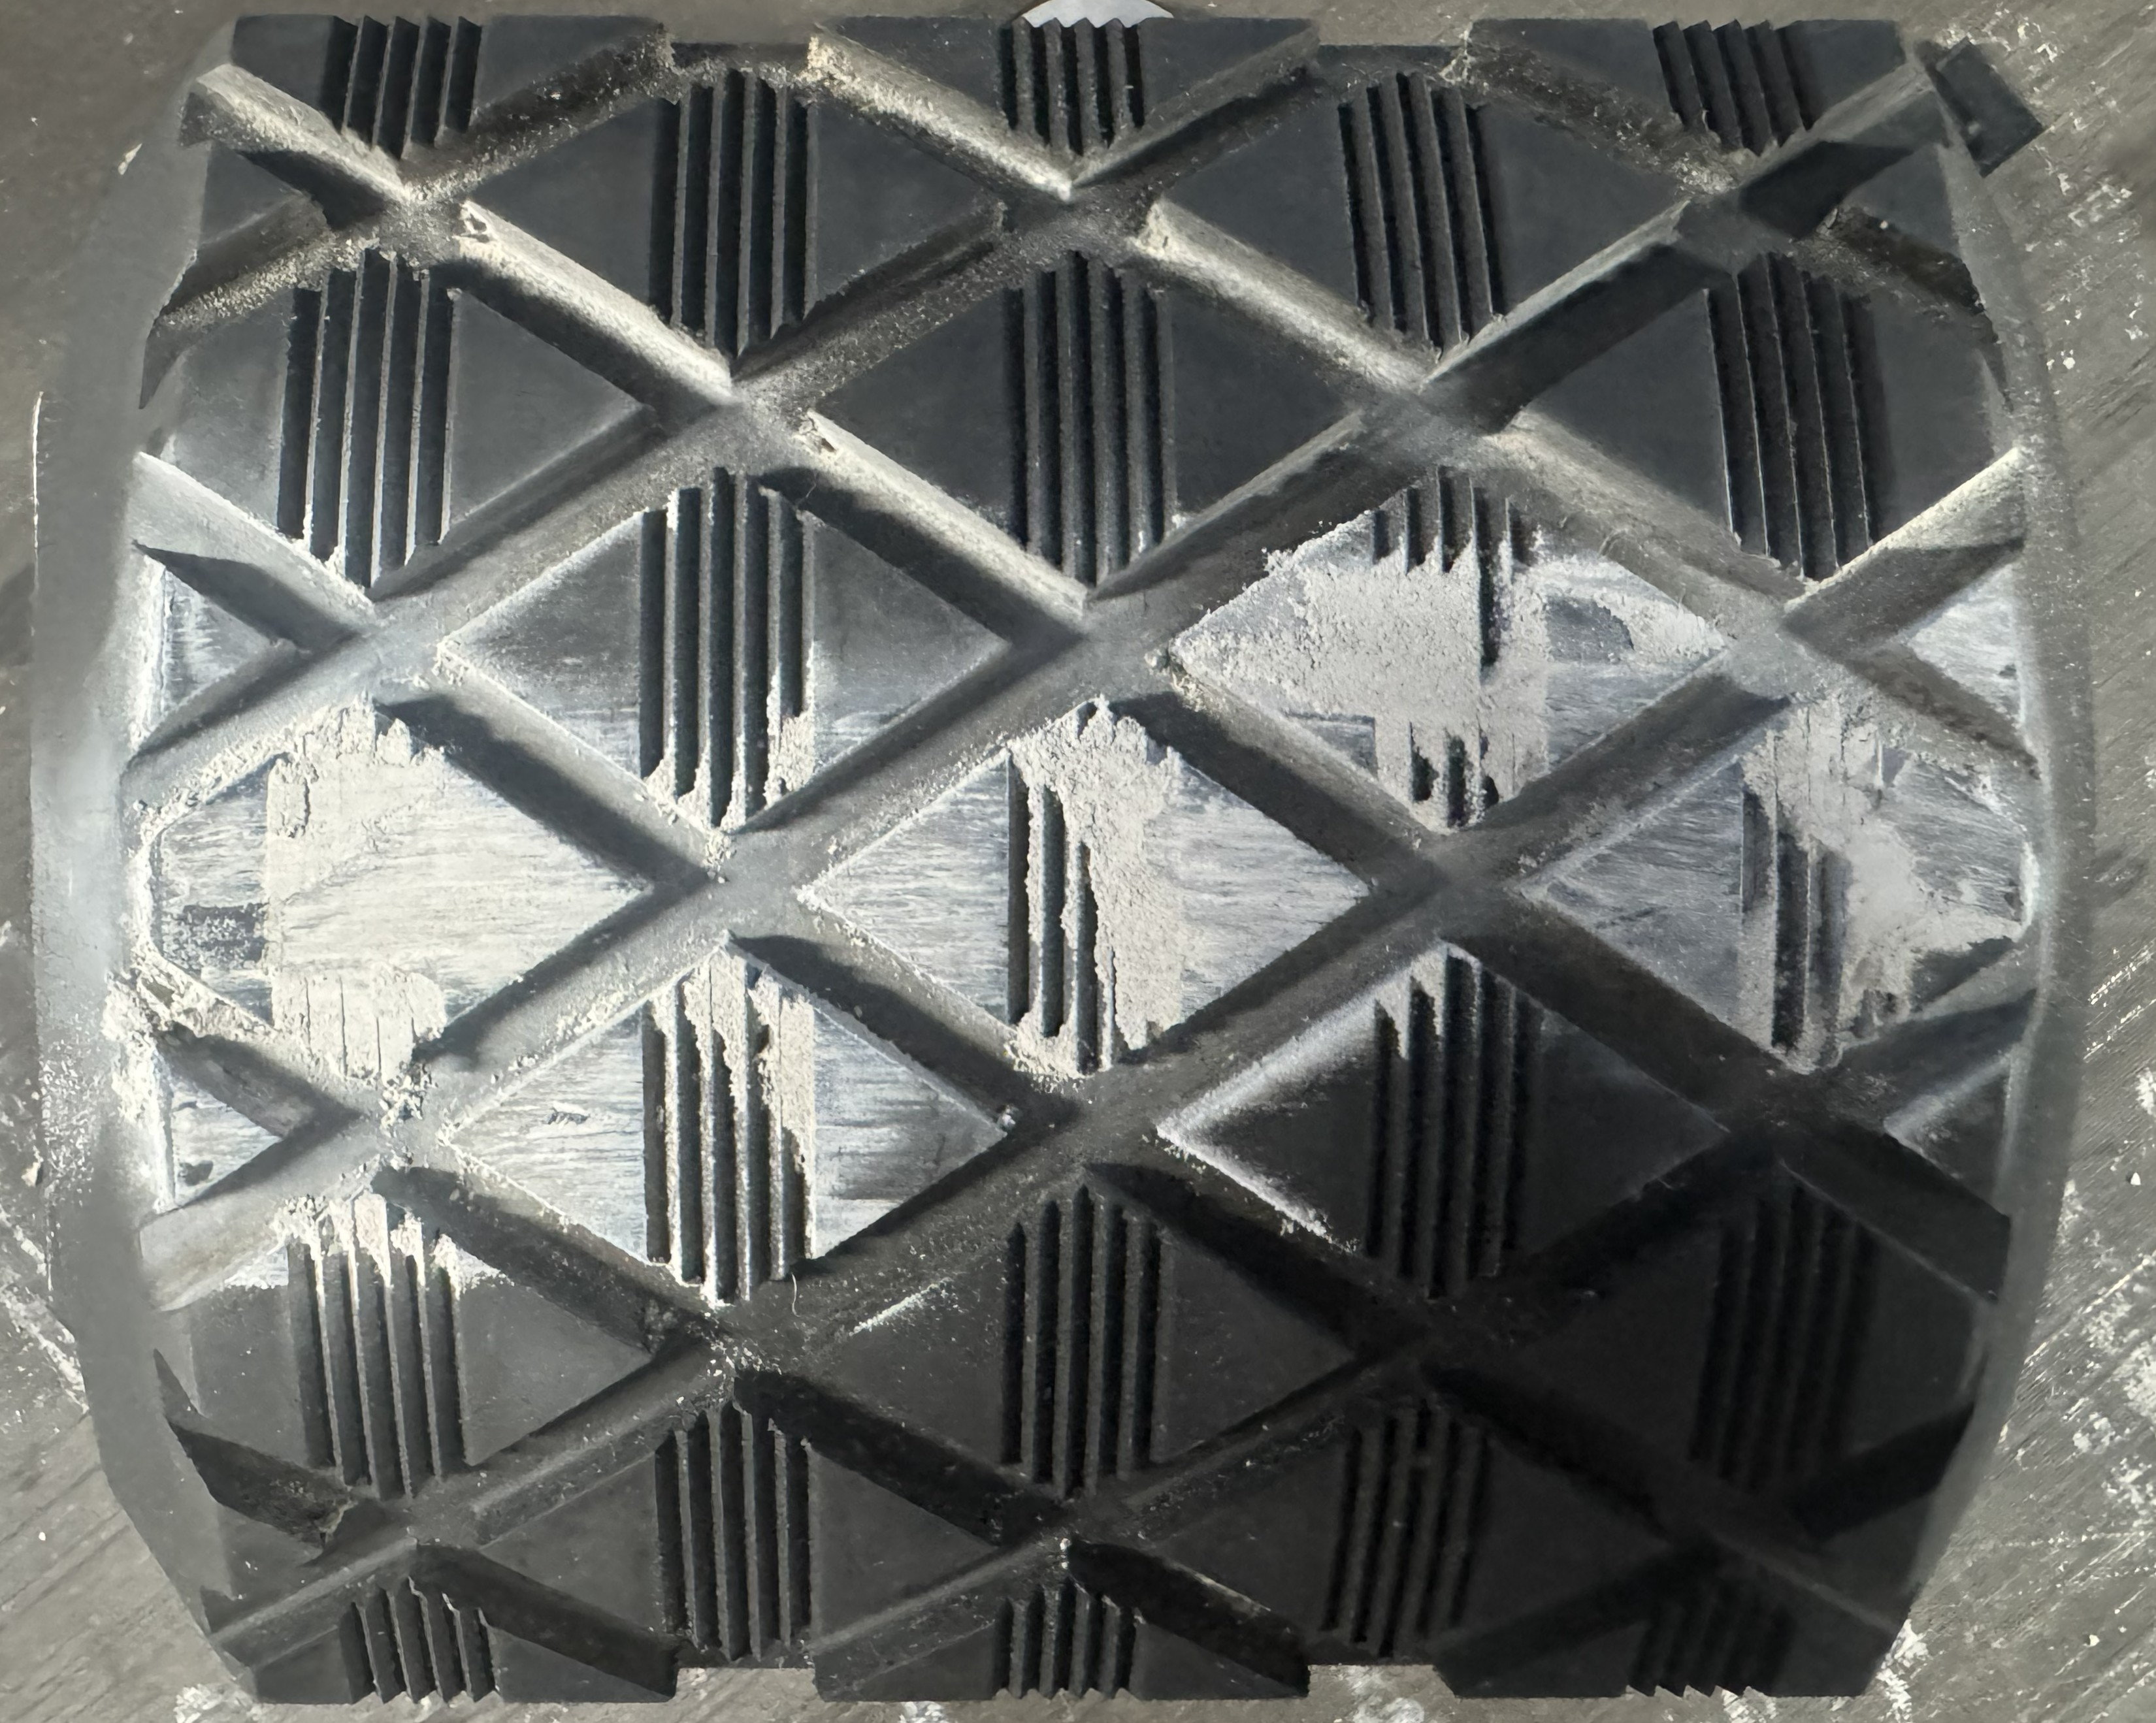
\includegraphics[width=.32\textwidth]{figure/chapter3/scraper-4.jpg}
	\label{fig:scraper_4}
	}
	\vspace{1em}
	\subfloat[$\delta_s=5.155\textrm{mm}$]{%
	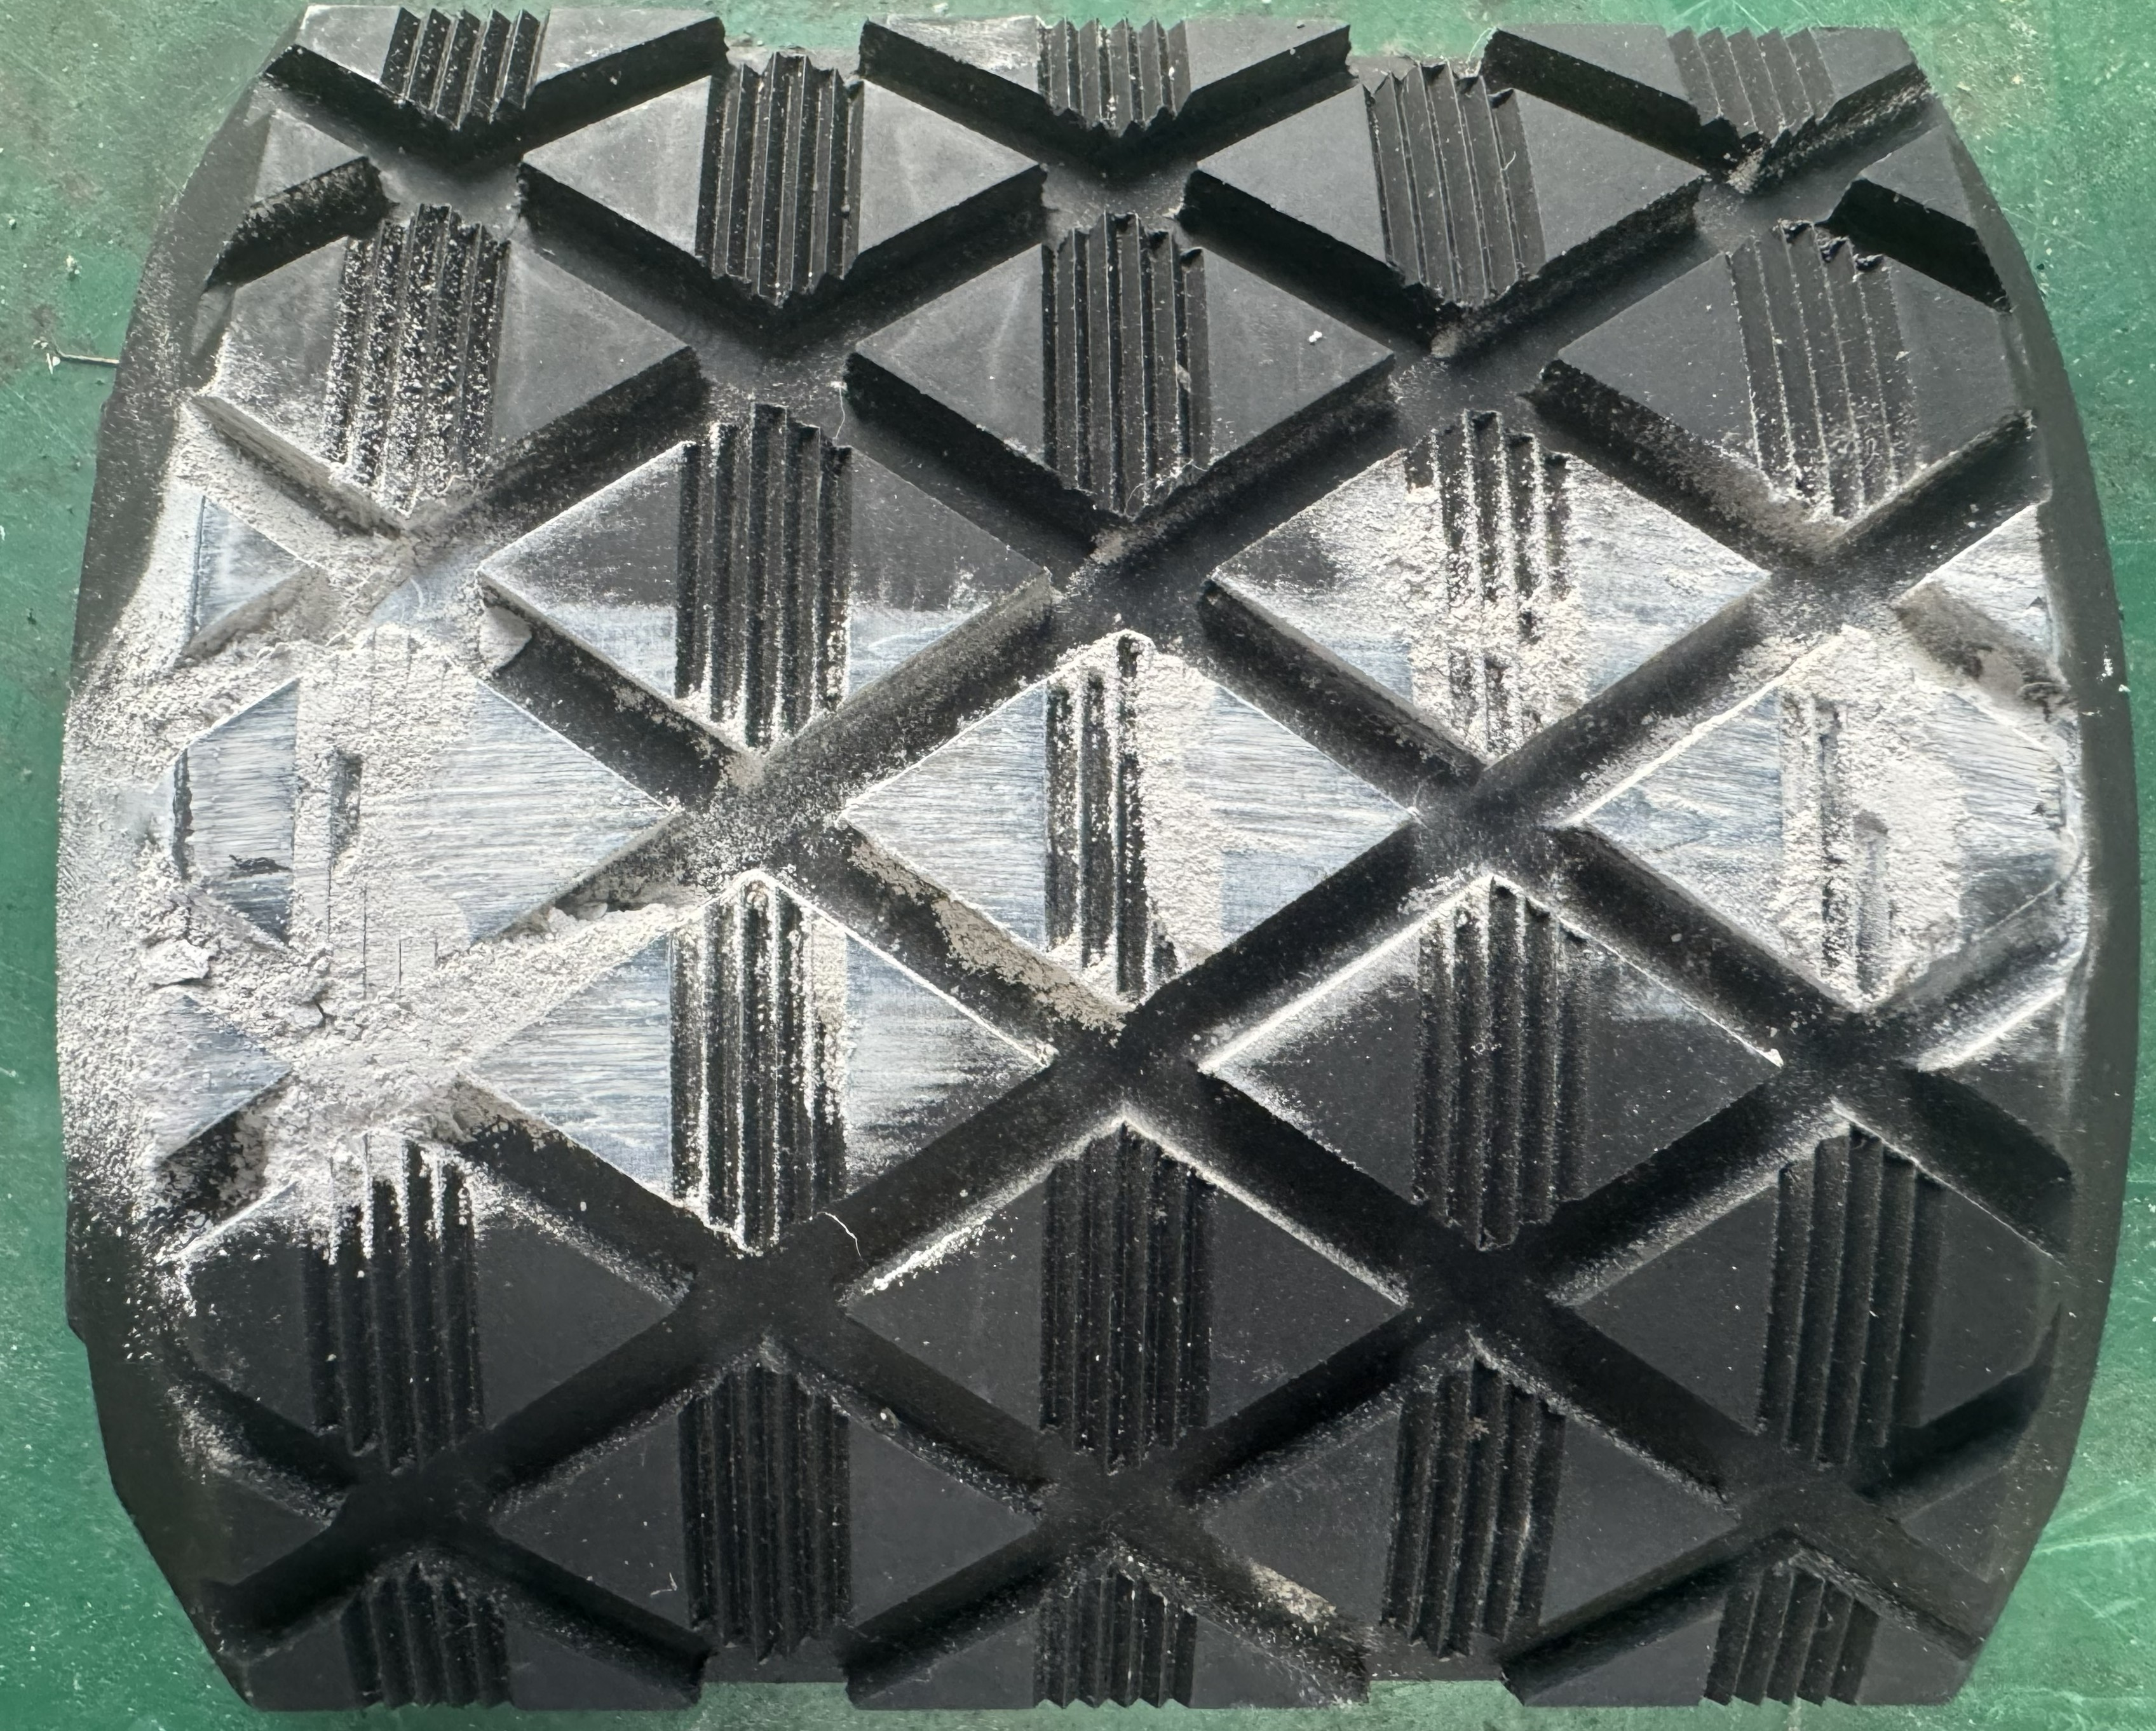
\includegraphics[width=.32\textwidth]{figure/chapter3/scraper-3.jpg}
	\label{fig:scraper_3}
	}
	%\hfill
	\subfloat[$\delta_s=6.465\textrm{mm}$]{%
	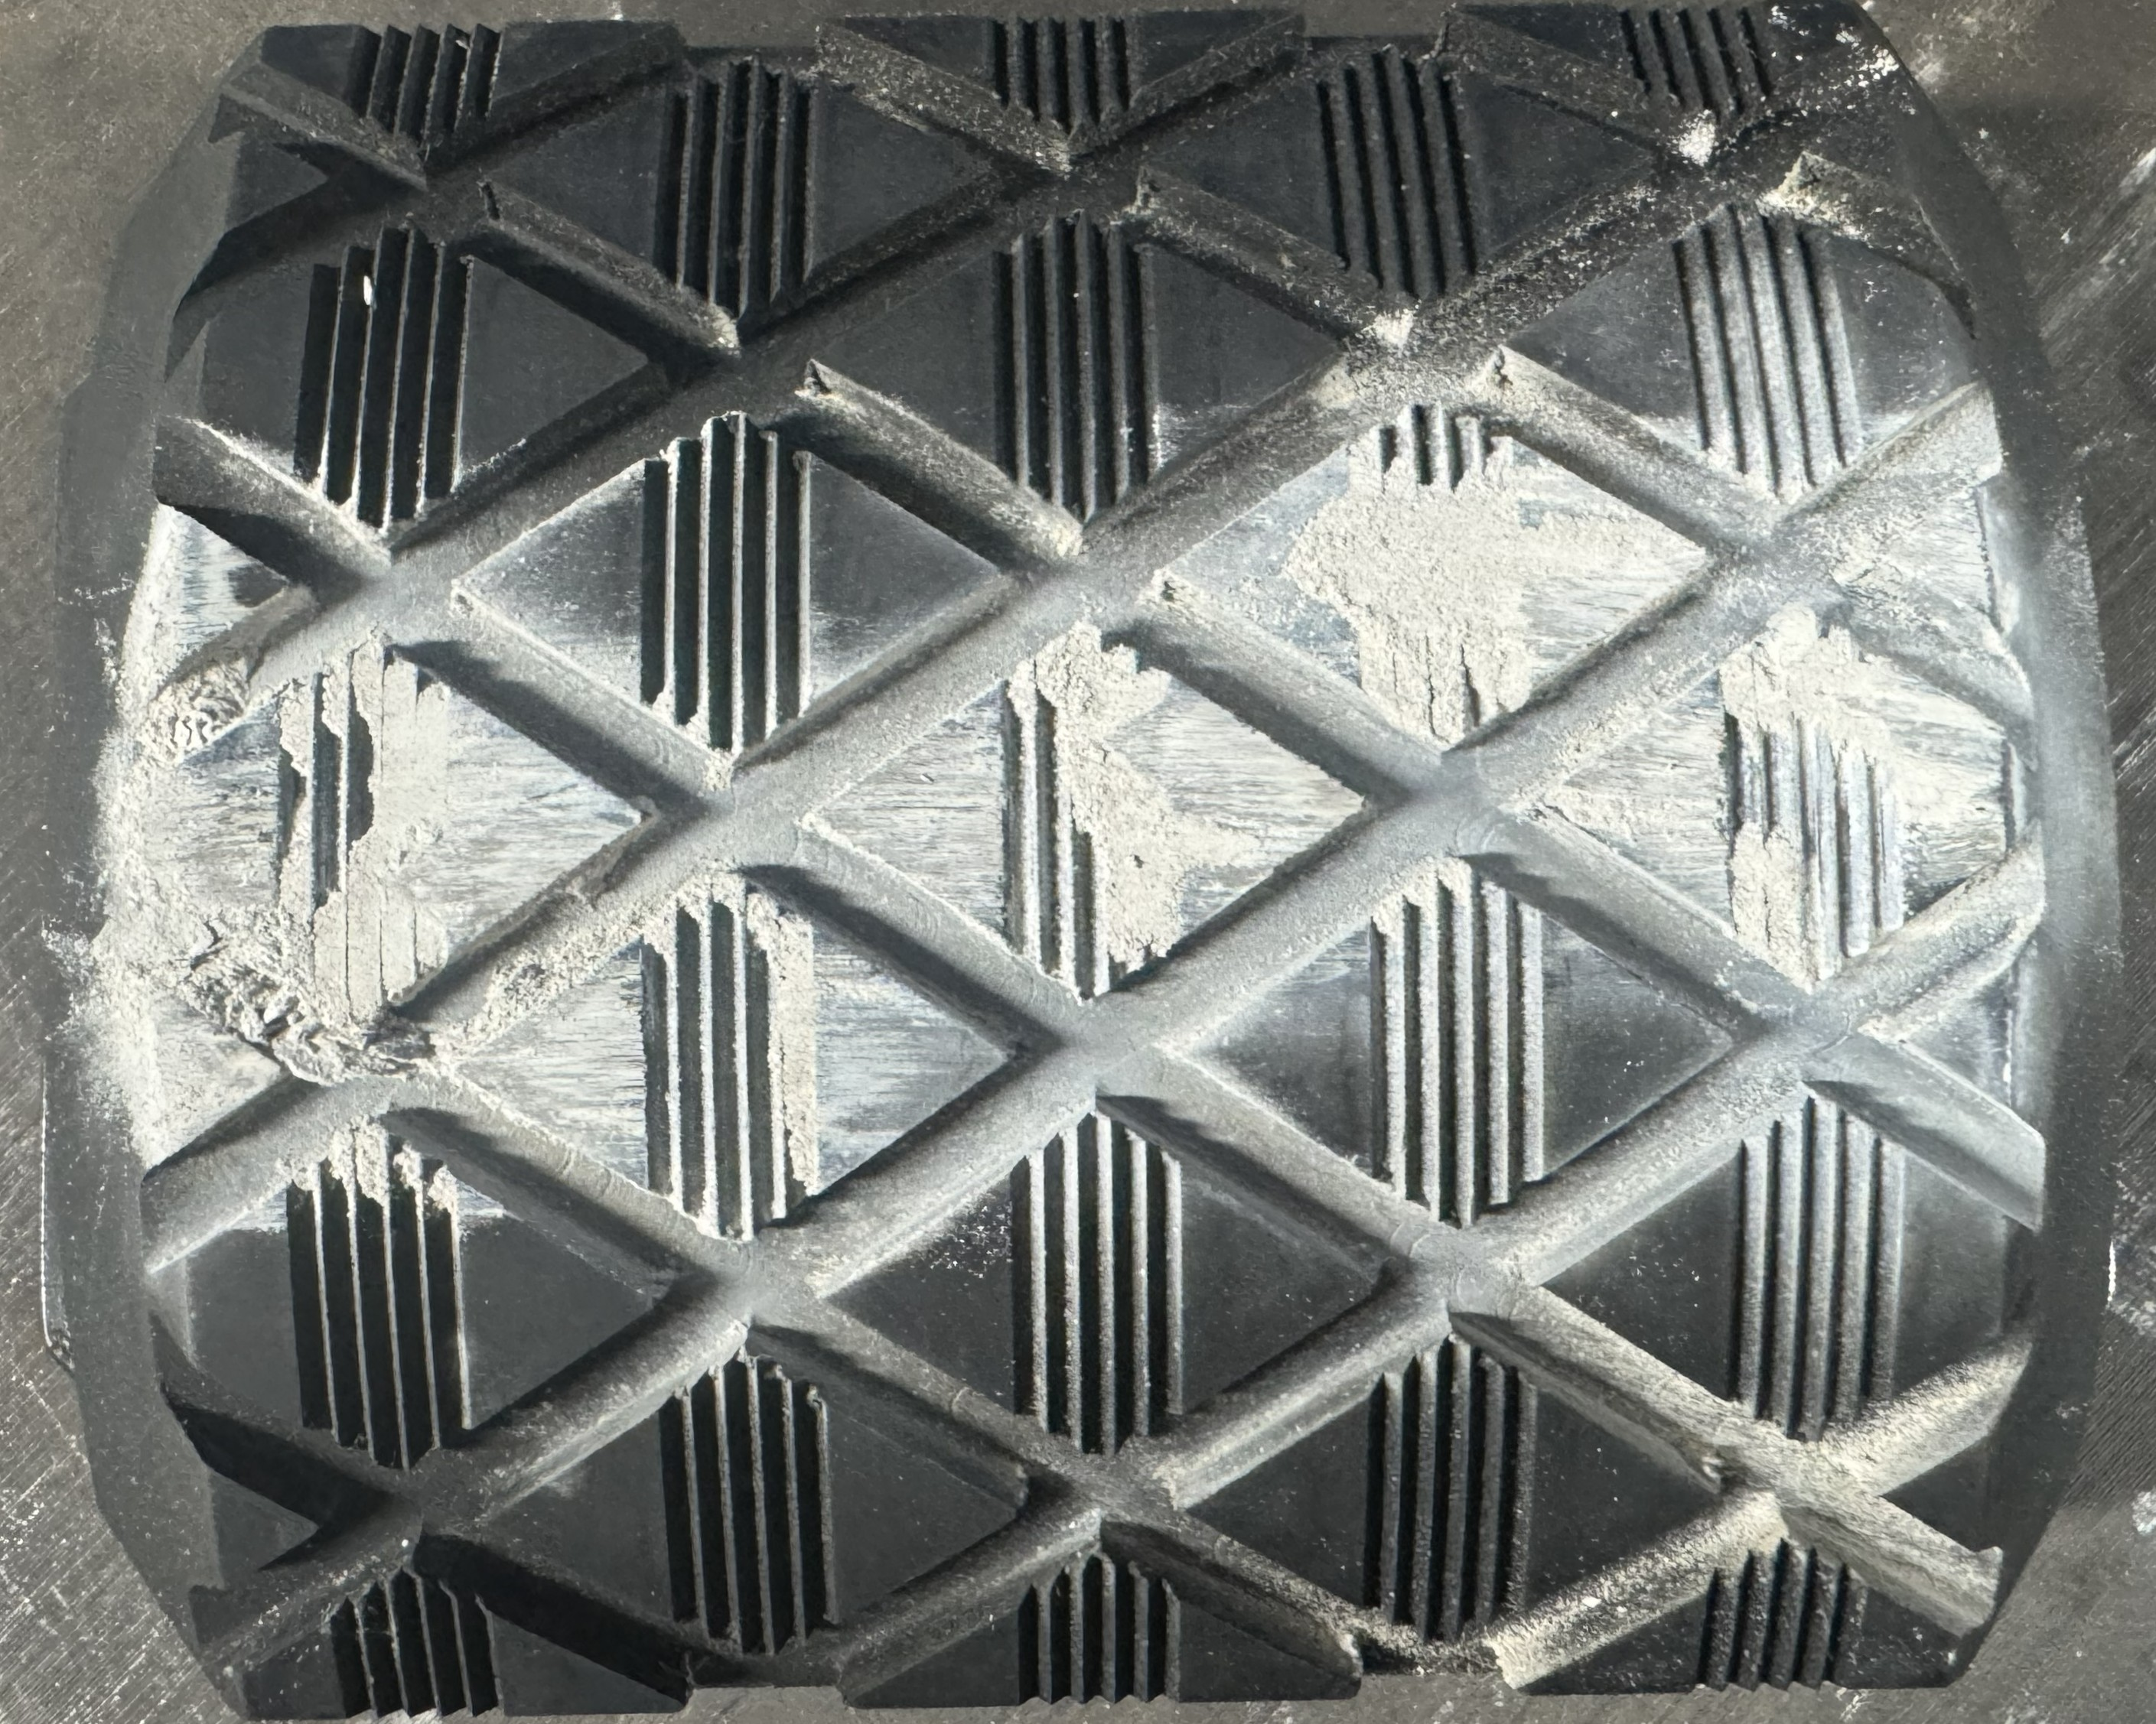
\includegraphics[width=.32\textwidth]{figure/chapter3/scraper-5.jpg}
	\label{fig:scaper_5}
	}	
	\caption{刮削后刮板刀齿表面形貌及切屑堵塞情况}
	\label{fig:scraper_profile}
\end{figure}



本试验基于图\ref{fig:scraper_test_rig}所示的转盘式台架，以重晶石粉与硫铝酸盐水泥配制的模拟硬垢为对象，考察了弹簧压缩量对刮板刮削效果的影响。结果表明：所设计的刮板能够有效刮除该类硬垢，但单次刮削厚度并不随弹簧预紧量的增大而增大，而是随弹簧压缩量的增大而减小，并在某一压缩量附近出现陡降，说明实际应用中弹簧预紧量存在临界值与有效工作区间。

从装置与方法看，转盘旋转可在低速条件下复现刮板相对垢面的刮削运动：接触区内相对运动方向与直线平动一致，线速度沿刮刀跨度虽有约±19\%的变化，但处于低速准静态范围，不改变硬垢脆性崩碎的去除机理；结合弹簧变形量与刮痕深度的逐点测量，可定量评价不同预紧工况下的刮削效果，为刮管工具的台架评价提供了可行方法。

从刮削形貌看，刮削后的垢面呈连续规则的沟槽，刀齿前刀面与容屑槽内见粉末状及崩碎状切屑（图\ref{fig:scale_profile}），表明垢层以脆性崩碎方式去除，刮板具备对重晶石/钡锶类硬垢的实际刮除能力；同时可见，产屑量随弹簧压缩量的增大而增多，而细屑对刀齿前刀面、容屑槽的充填堵塞及垢面压实变质层的发育也随压缩量的增大而加剧（图\ref{fig:scraper_profile}），说明单纯增大预紧量并不能成比例地提高有效刮削能力，这与图\ref{fig:scratch_depth_spring_comprassion}所示的响应规律一致。

从单次刮削厚度随弹簧压缩估计值的响应看（图\ref{fig:scratch_depth_spring_comprassion}），二者并非单调递增关系，而呈“缓降—陡降—稳定”的三段特征：弹簧压缩量约为3.9 mm和5.5 mm时，单次刮削厚度分别约为0.85 mm和0.71 mm，降幅不大；压缩量增至约7.1 mm时，厚度约为0.64 mm；压缩量进一步增至约7.3 mm时，厚度骤降至约0.11 mm；此后（约9.6 mm）厚度基本稳定在0.08 mm左右。由此可知，弹簧预紧量存在临界值（本试验条件下约为7.2 mm）：在临界值以内，刀齿能够保持相对稳定的压入深度，单次刮削厚度随压缩量的增大缓慢减小；当压缩量接近并超过临界值后，一方面刀齿与垢面的实际接触面积显著增大、垢层表面被压实变质并产生大量细屑，细屑迅速充填刀齿前刀面与容屑槽（图\ref{fig:scraper_profile}），参与有效切削的齿减少；另一方面刮板的浮动支撑逐渐接近其径向行程极限，刀齿难以继续压入垢层，刮削中切削所占比重下降、挤压与摩擦所占比重上升，单次刮削厚度急剧下降并趋于稳定。需要说明的是，本文各工况在同一扇形垢样、同一沟槽上依次进行，弹簧压缩量随工况逐步调整，图中反映的是弹簧压缩量对刮削厚度的总体影响趋势。

面向工程应用，弹簧预紧量不宜盲目加大，而应控制在其有效区间内：预紧量过小，刀齿难以始终贴紧壁面，清洁能力受限；预紧量过大，单次刮削厚度不升反降，并会因齿面堵塞和浮动支撑压死使刮削能力骤降，同时加剧刀齿与后刀面的磨损。按本节试验结果，弹簧压缩量在约4$\sim$7 mm范围内时，单次刮削厚度保持在较高水平且变化平缓，可作为该刮板预紧量的推荐工作区间；实际应用中还应结合套管的实际内径（同一公称尺寸不同线重时内径不同）匹配刮刀外径与弹簧预紧量，使弹簧压缩量不超过临界值，避免盲目增大预紧力；现场作业宜配合循环冲洗及时排屑，以延缓齿面堵塞、延长刮板有效使用寿命。

综上，研制的刮板对重晶石/钡锶类硬垢刮削有效，转盘台架及其测量方法可用于刮板刮削能力的相对评价；单次刮削厚度随弹簧压缩量的增大而减小，并在约7.2 mm附近出现陡降，说明弹簧预紧量存在临界值，实际应用中应结合套管规格匹配刮刀外径与弹簧预紧量、将弹簧压缩量控制在临界值以内，并辅以循环排屑措施。
\begin{figure}	
	\centering
	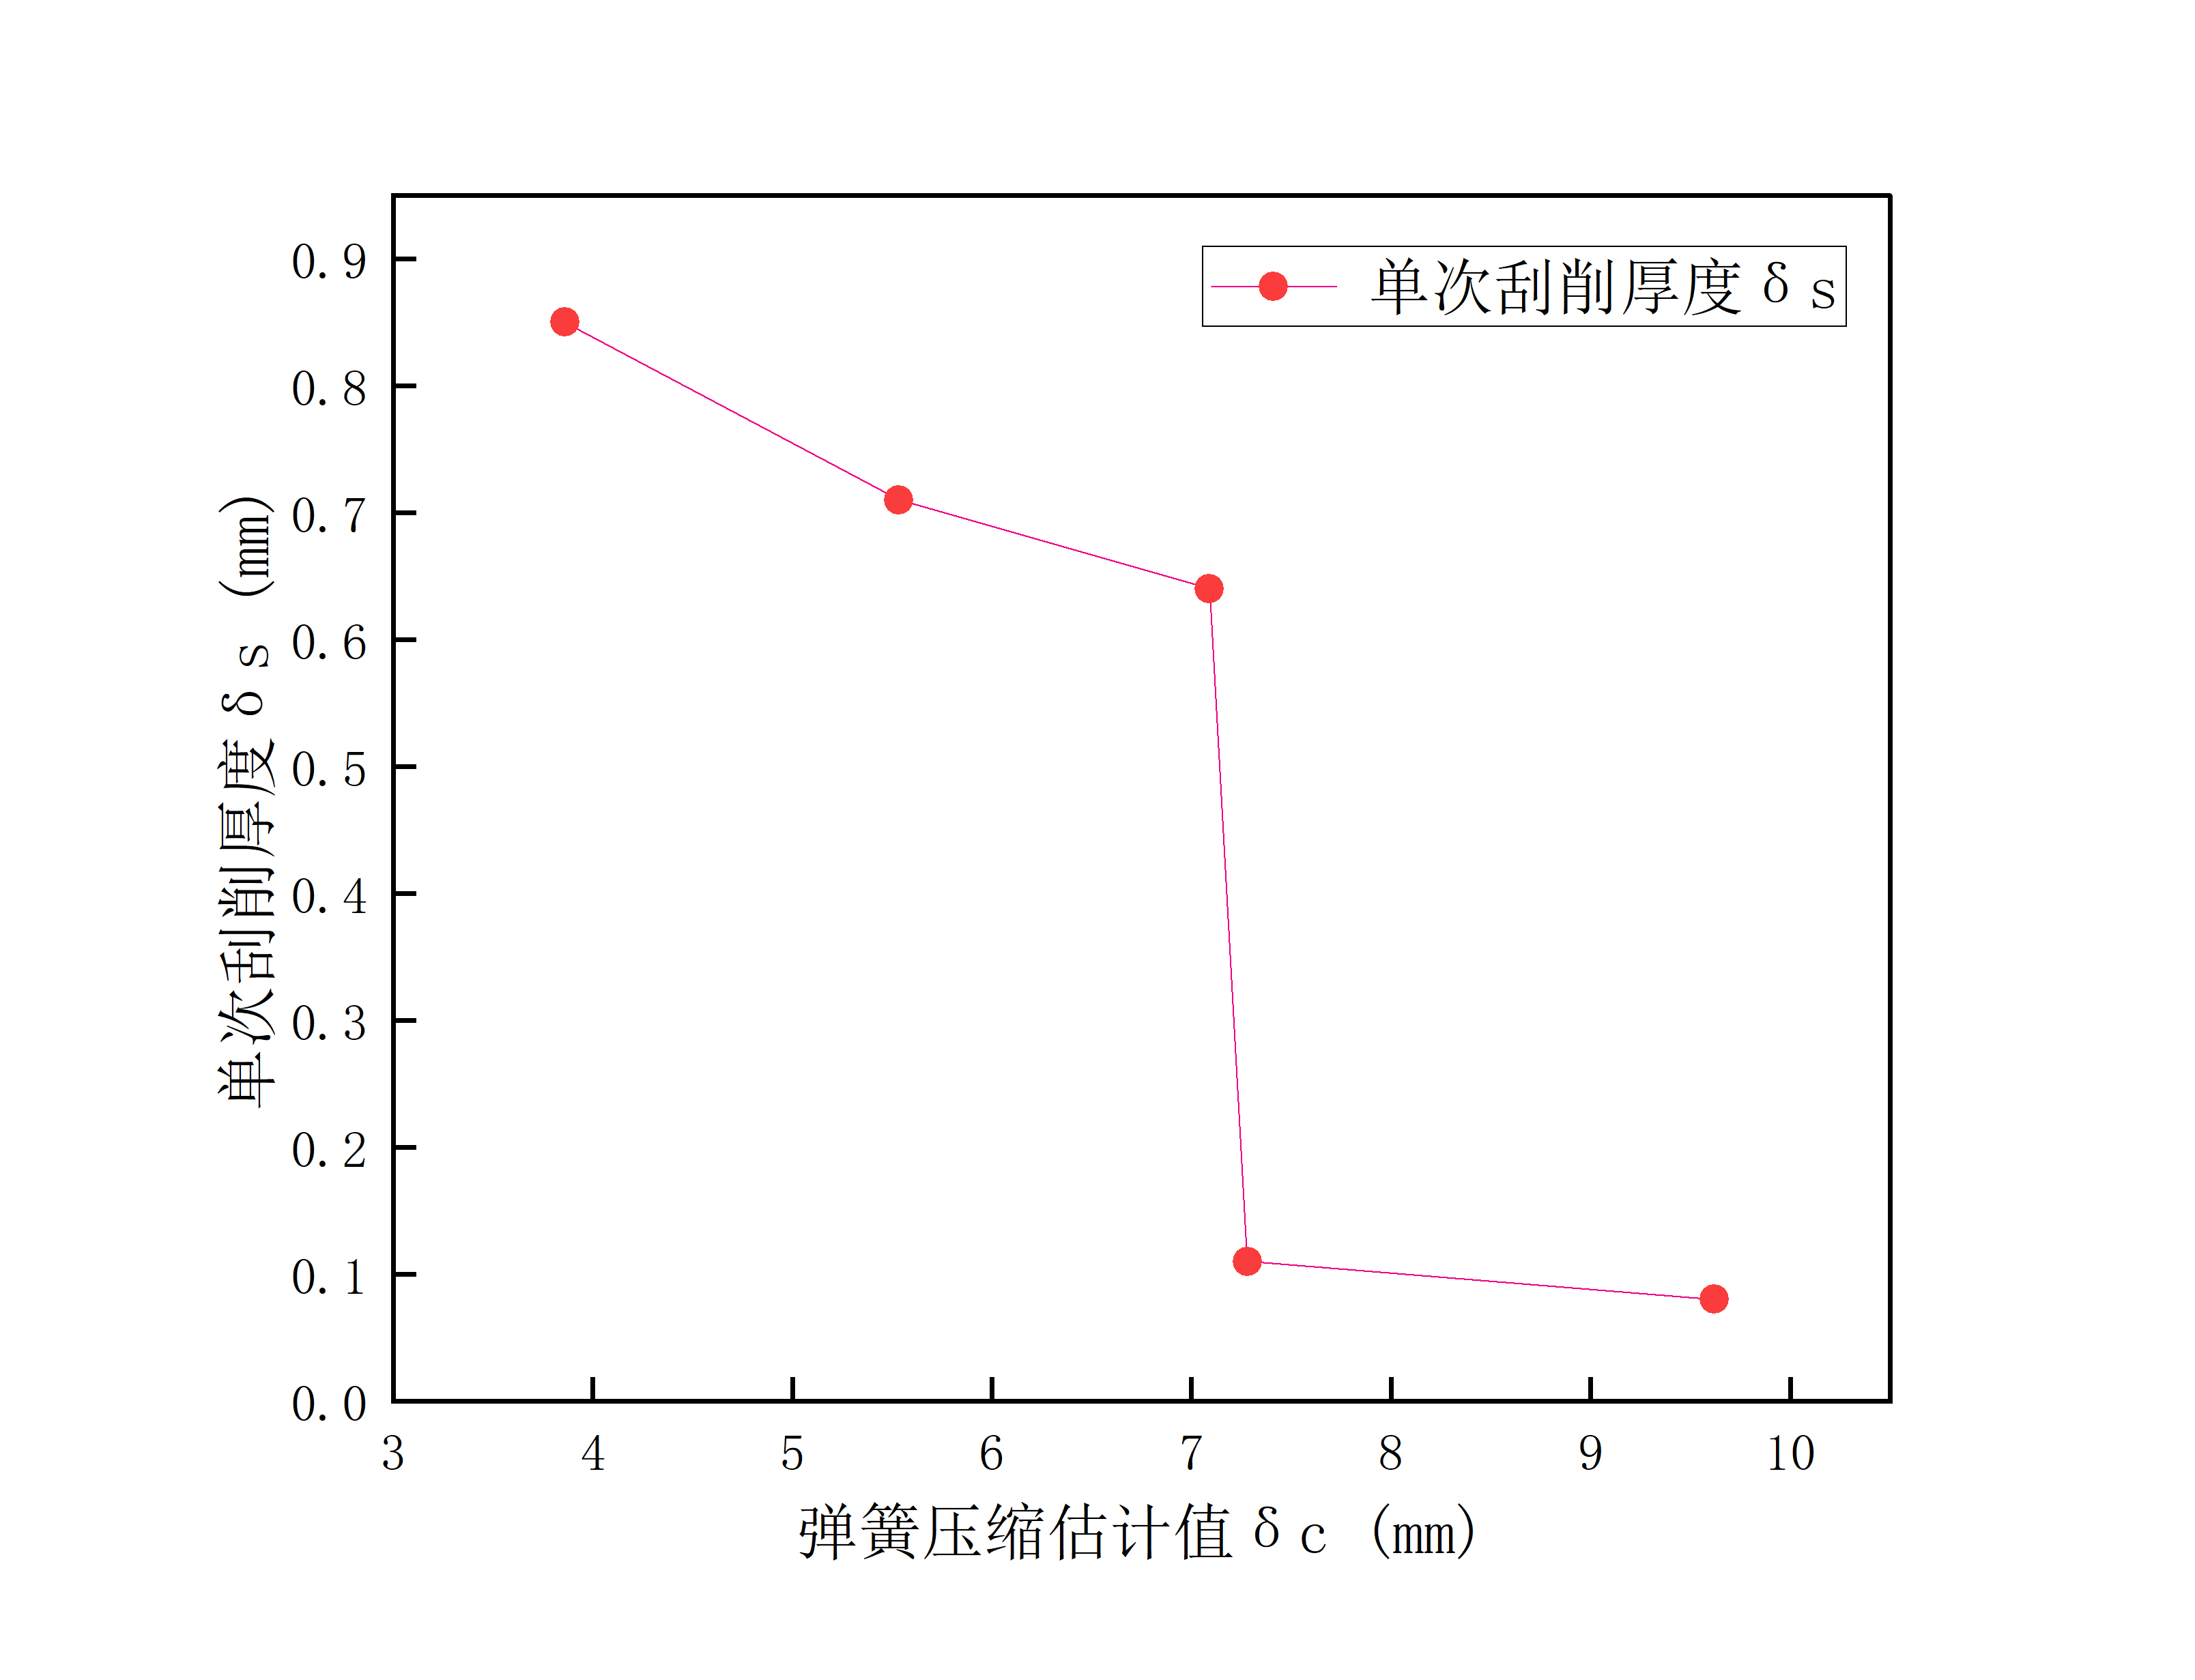
\includegraphics[width=.7\textwidth]{figure/chapter3/scatch-depth-sping-comprassion.jpg}
	\caption{刮削深度与弹簧压缩量之间的关系}
	\label{fig:scratch_depth_spring_comprassion}
\end{figure}


%\subsection{毛刷刮削力学仿真}


\subsection{操作方式}
\subsubsection{ 使用方法}
根据井眼尺寸选择合适的套管清洁工具，根据井眼情况选择各模块的数量及排列组合方式。
四合一工具用钻柱送入井底进行清洁作业。
\subsubsection{ 操作方法}
该工具可以与强磁吸附工具一同使用（推荐），也可以单独使用。
将四合一工具下到井底离通井位置$\mathrm{3-5m}$处，开泵循环。将四合一工具在该位置上下活动。保持循环的情况下，平稳的上体钻柱。
起钻时要求平稳、低速、严禁剧烈震动与撞击。

\subsection{维护与保养}
\subsubsection{保养}
下井使用过的四合一工具必须进行保养及维修，在钻台现场进 行保养是在井场钻台上起出井后，四合一工具外表面和水眼内的泥浆。

\subsubsection{管子站维修}
建议：在井下正常运转400小时后的四合一工具应送管子站进行大修，必须更换所有密封件和易损件，工具大修三次后报废。外筒零件磨损量（或偏磨量）大于产品外径尺寸1\%时，该套管清洁工具报废。修前应准备好下列设备、工具、附件：适用于该工具尺寸的链钳、管钳、手钳等相应工具；起重吊车、固定钳、稳定座、拆装架，试验架等设备；清洗用的煤油等；各种所需的润滑脂、润滑油等。

\subsection{测试与检查}

刮削器所用金属材料如需作力学性能试验，应按GB/T228的有关规定进行。刮板寿命按照SY/T 5110-2000进行刮刀寿命测试，刮削器的刮削寿命试验应在模拟试验台上进行。选用500号硅酸盐水泥，在对应的试验套管内壁上候凝24h。将试验套管固定在试验台底座上，将刮削器接到试验台的钻杆上，加压力$0.8~10\mathrm{kN}$，用$36\mathrm{r/min}$的速度进行模拟刮削，每次刮削1h，刮削3次。然后拆检测量刀体的磨损量，用渐进法验证其寿命。

四合一工具拆卸后应尽快进行检查，更换不满足使用条件的配件，不能采用非原厂配件。清洗前的检查，肉眼检查外部零件的损坏并记录异常磨损或作记号。如果发现明显损伤，需要对配件进行特别处理。清洗，用水浸泡零件以除掉干的结块和泥浆。用蒸汽和强力生物清洁剂去掉油和黄油。配件干燥、冷却后进行检查。

每次套管清洁工具被拆开时，用下述步骤检查所有配件。按API标准检查所有的接头螺纹，检查步骤要符合API标准。检查所有的配合面和端面是否清洗和磨损，需要时，修理和更换配件。检查所有外部配件是否磨损，当外径磨损超过尺寸的1\%以上时， 更换配件。配件有超过最小磨损量的凹槽或缺口不能继续使用，在一个小区域有许多凹槽 或缺口也不能再使用，要求更换配件。探伤检查，每次维修时，对所有受力件进行超声波或磁粉探伤检查，如果发现裂缝和伤痕指示，而且不能被修复的，则更换配件。用新、修理过的或继续使用的配件进行装配。所有配件须保证整洁。

